\documentclass[11pt]{article}
\usepackage[textwidth=18.0cm, textheight=23.0cm, top=2.0cm]{geometry}
\usepackage{pst-all}
\usepackage{amssymb}
\usepackage{tikz}
\usepackage{underscore}\begin{document}
\pagestyle{empty}


ClassName: \underline{\textbf{Class_05.2bp-31}}
\par
BinSize: \underline{\textbf{100 × 100}}
\par
ReduceSize: \underline{\textbf{100 × 100}}
\par
TypeNum: \underline{\textbf{80}}
\par
Num: \underline{\textbf{80}}
\par
OutS: \underline{\textbf{230000}}
\par
InS: \underline{\textbf{200789}}
\par
Rate: \underline{\textbf{0.873}}
\par
UB: \underline{\textbf{23}}
\par
LB0: \underline{\textbf{23}}
\par
LB: \underline{\textbf{23}}
\par
LBWithCut: \underline{\textbf{23}}
\par
NodeCut: \underline{\textbf{0}}
\par
ExtendedNodeCnt: \underline{\textbf{1}}
\par
GenNodeCnt: \underline{\textbf{1}}
\par
PrimalNode: \underline{\textbf{0}}
\par
ColumnCount: \underline{\textbf{23}}
\par
TotalCutCount: \underline{\textbf{0}}
\par
RootCutCount: \underline{\textbf{0}}
\par
LPSolverCnt: \underline{\textbf{1}}
\par
PricingSolverCnt: \underline{\textbf{0}}
\par
BranchAndBoundNum: \underline{\textbf{1}}
\par
isOpt: \underline{\textbf{true}}
\par
TimeOnInitSolution: \underline{\textbf{600.000 s}}
\par
TimeOnPrimal: \underline{\textbf{0.000 s}}
\par
TimeOnPricing: \underline{\textbf{0.000 s}}
\par
TimeOnRmp: \underline{\textbf{0.062 s}}
\par
TotalTime: \underline{\textbf{600.328 s}}
\par
\newpage


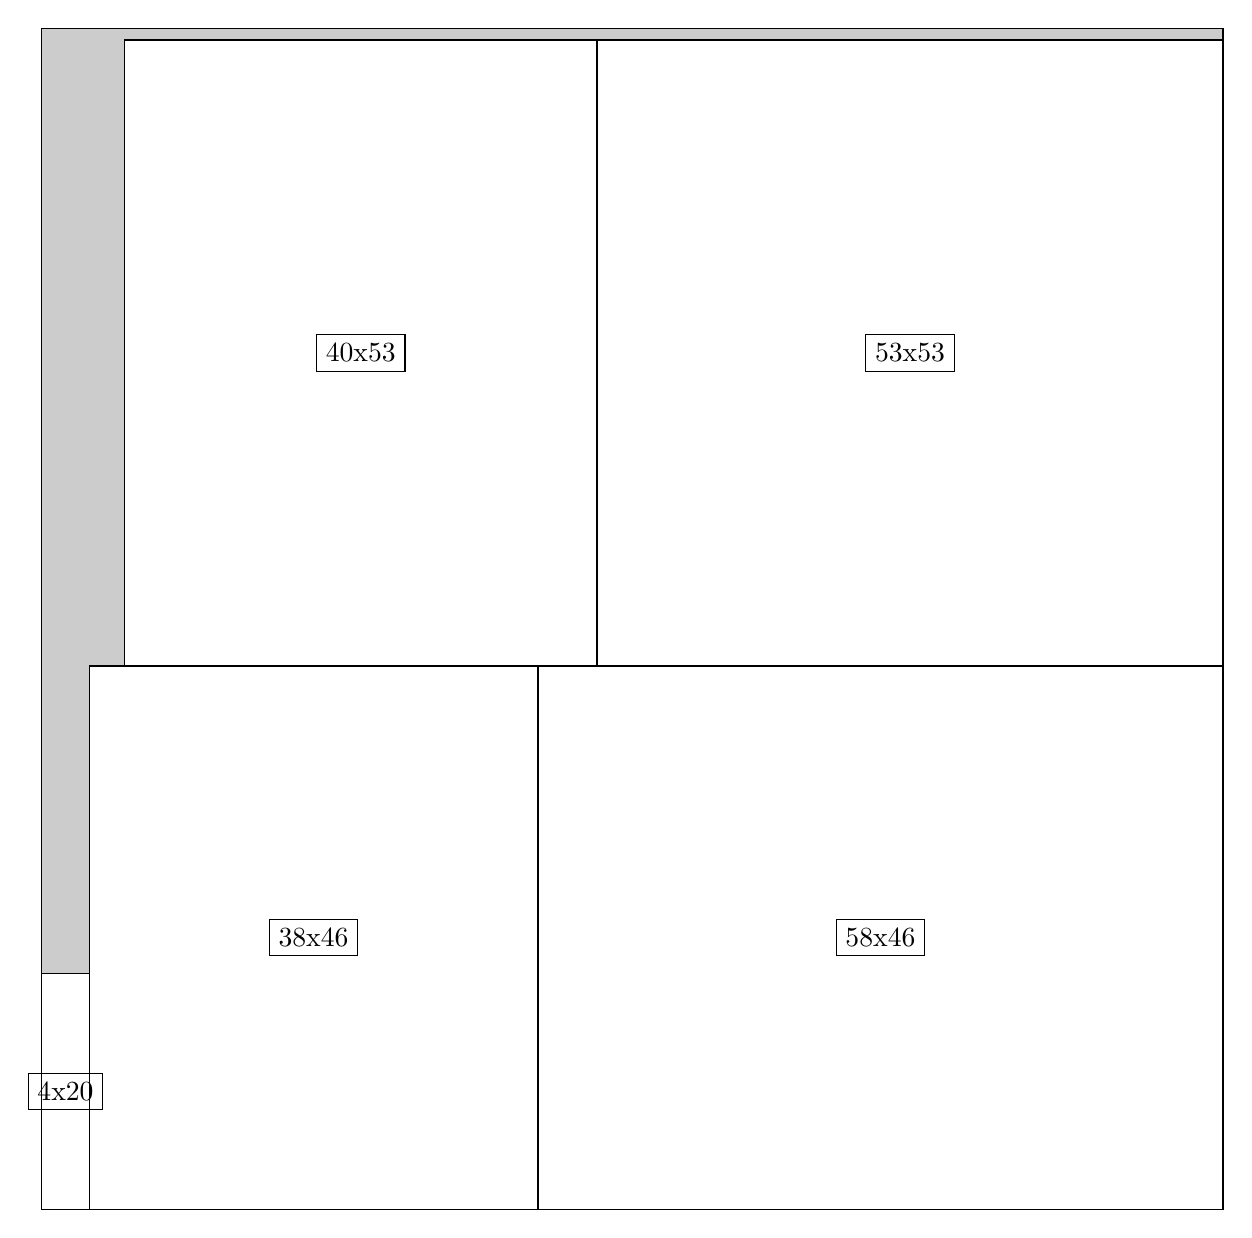
\begin{tikzpicture}[shorten >=1pt,scale=1.0,every node/.style={scale=1.0},->]
\tikzstyle{vertex}=[circle,fill=black!25,minimum size=14pt,inner sep=0pt]
\filldraw[fill=gray!40!white, draw=black] (0,0) rectangle (15.0,15.0);
\foreach \name/\x/\y/\w/\h in {58x46/6.3/0.0/8.7/6.8999999999999995,38x46/0.6/0.0/5.7/6.8999999999999995,4x20/0.0/0.0/0.6/3.0,53x53/7.05/6.8999999999999995/7.949999999999999/7.949999999999999,40x53/1.05/6.8999999999999995/6.0/7.949999999999999}
\filldraw[fill=white!40!white, draw=black] (\x,\y) rectangle node[draw] (\name) {\name} ++(\w,\h);
\end{tikzpicture}


w =58 , h =46 , x =42 , y =0 , v =2668
\par
w =38 , h =46 , x =4 , y =0 , v =1748
\par
w =4 , h =20 , x =0 , y =0 , v =80
\par
w =53 , h =53 , x =47 , y =46 , v =2809
\par
w =40 , h =53 , x =7 , y =46 , v =2120
\par
\newpage



\begin{tikzpicture}[shorten >=1pt,scale=1.0,every node/.style={scale=1.0},->]
\tikzstyle{vertex}=[circle,fill=black!25,minimum size=14pt,inner sep=0pt]
\filldraw[fill=gray!40!white, draw=black] (0,0) rectangle (15.0,15.0);
\foreach \name/\x/\y/\w/\h in {97x93/0.44999999999999996/0.0/14.549999999999999/13.95}
\filldraw[fill=white!40!white, draw=black] (\x,\y) rectangle node[draw] (\name) {\name} ++(\w,\h);
\end{tikzpicture}


w =97 , h =93 , x =3 , y =0 , v =9021
\par
\newpage



\begin{tikzpicture}[shorten >=1pt,scale=1.0,every node/.style={scale=1.0},->]
\tikzstyle{vertex}=[circle,fill=black!25,minimum size=14pt,inner sep=0pt]
\filldraw[fill=gray!40!white, draw=black] (0,0) rectangle (15.0,15.0);
\foreach \name/\x/\y/\w/\h in {98x76/0.3/0.0/14.7/11.4}
\filldraw[fill=white!40!white, draw=black] (\x,\y) rectangle node[draw] (\name) {\name} ++(\w,\h);
\end{tikzpicture}


w =98 , h =76 , x =2 , y =0 , v =7448
\par
\newpage


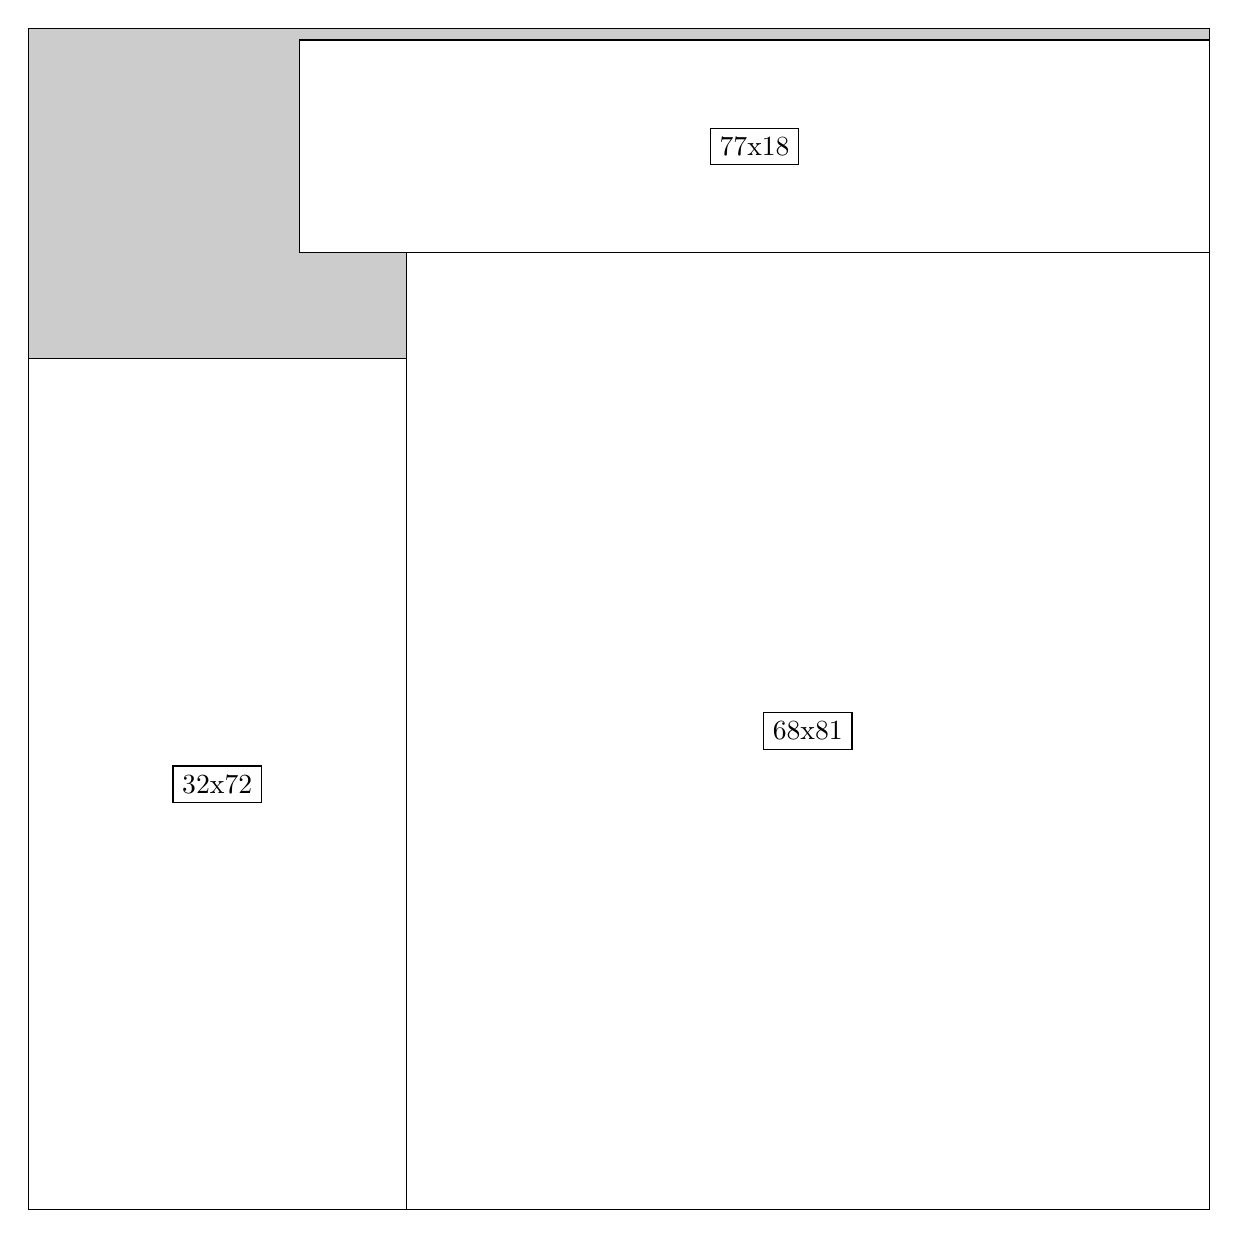
\begin{tikzpicture}[shorten >=1pt,scale=1.0,every node/.style={scale=1.0},->]
\tikzstyle{vertex}=[circle,fill=black!25,minimum size=14pt,inner sep=0pt]
\filldraw[fill=gray!40!white, draw=black] (0,0) rectangle (15.0,15.0);
\foreach \name/\x/\y/\w/\h in {68x81/4.8/0.0/10.2/12.15,32x72/0.0/0.0/4.8/10.799999999999999,77x18/3.4499999999999997/12.15/11.549999999999999/2.6999999999999997}
\filldraw[fill=white!40!white, draw=black] (\x,\y) rectangle node[draw] (\name) {\name} ++(\w,\h);
\end{tikzpicture}


w =68 , h =81 , x =32 , y =0 , v =5508
\par
w =32 , h =72 , x =0 , y =0 , v =2304
\par
w =77 , h =18 , x =23 , y =81 , v =1386
\par
\newpage


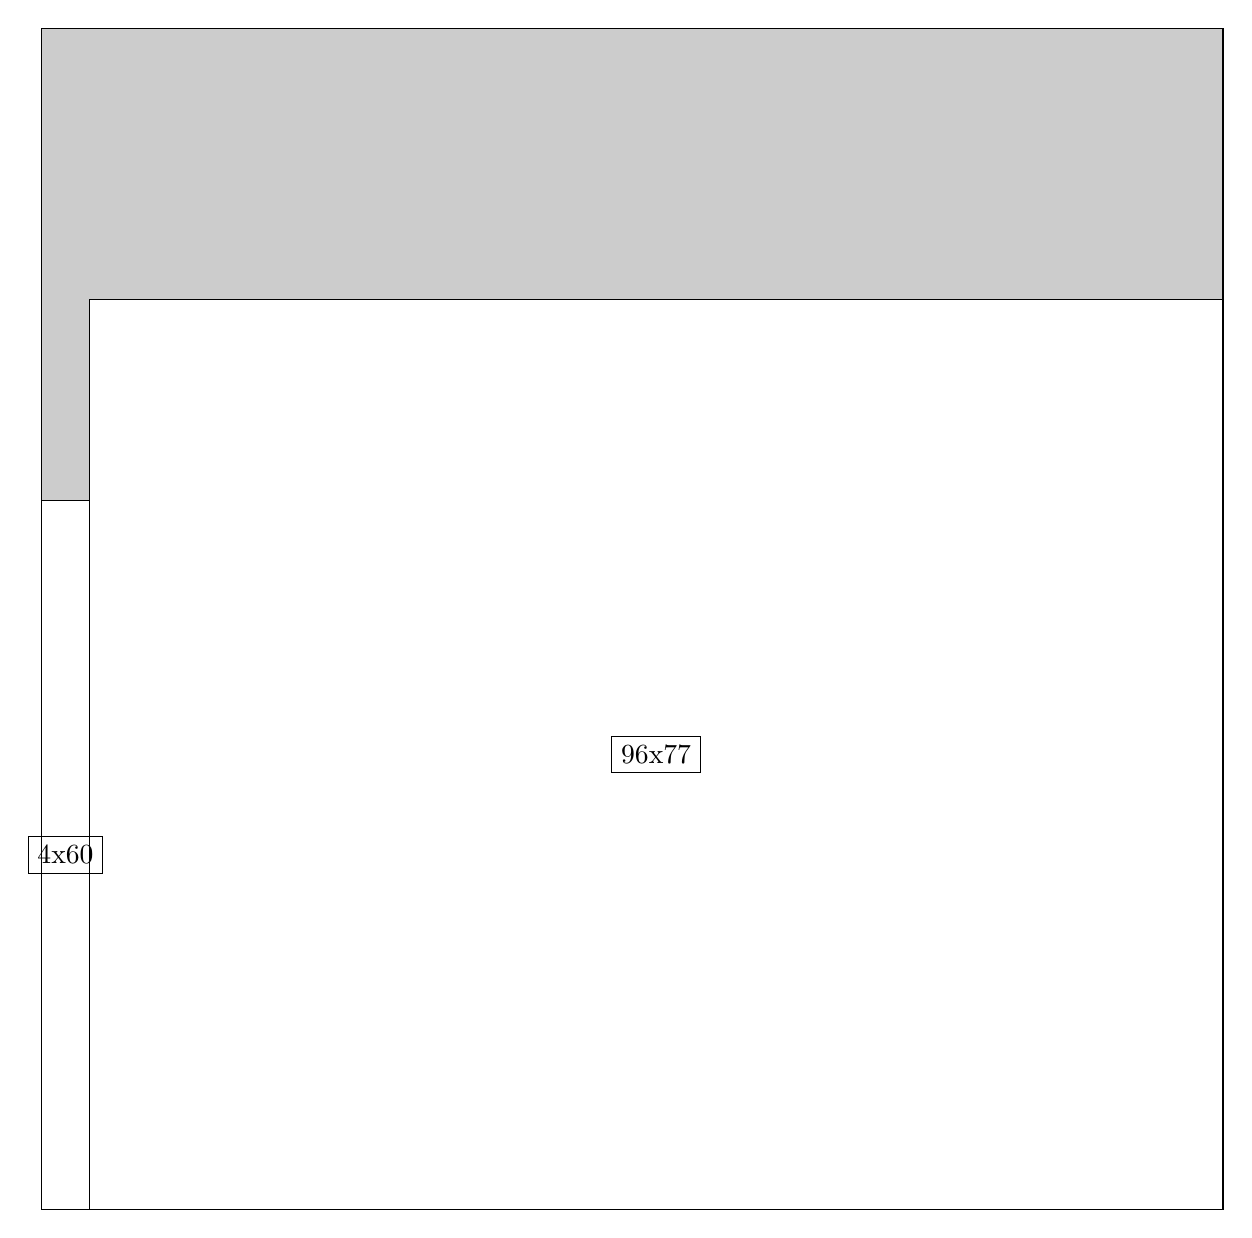
\begin{tikzpicture}[shorten >=1pt,scale=1.0,every node/.style={scale=1.0},->]
\tikzstyle{vertex}=[circle,fill=black!25,minimum size=14pt,inner sep=0pt]
\filldraw[fill=gray!40!white, draw=black] (0,0) rectangle (15.0,15.0);
\foreach \name/\x/\y/\w/\h in {96x77/0.6/0.0/14.399999999999999/11.549999999999999,4x60/0.0/0.0/0.6/9.0}
\filldraw[fill=white!40!white, draw=black] (\x,\y) rectangle node[draw] (\name) {\name} ++(\w,\h);
\end{tikzpicture}


w =96 , h =77 , x =4 , y =0 , v =7392
\par
w =4 , h =60 , x =0 , y =0 , v =240
\par
\newpage


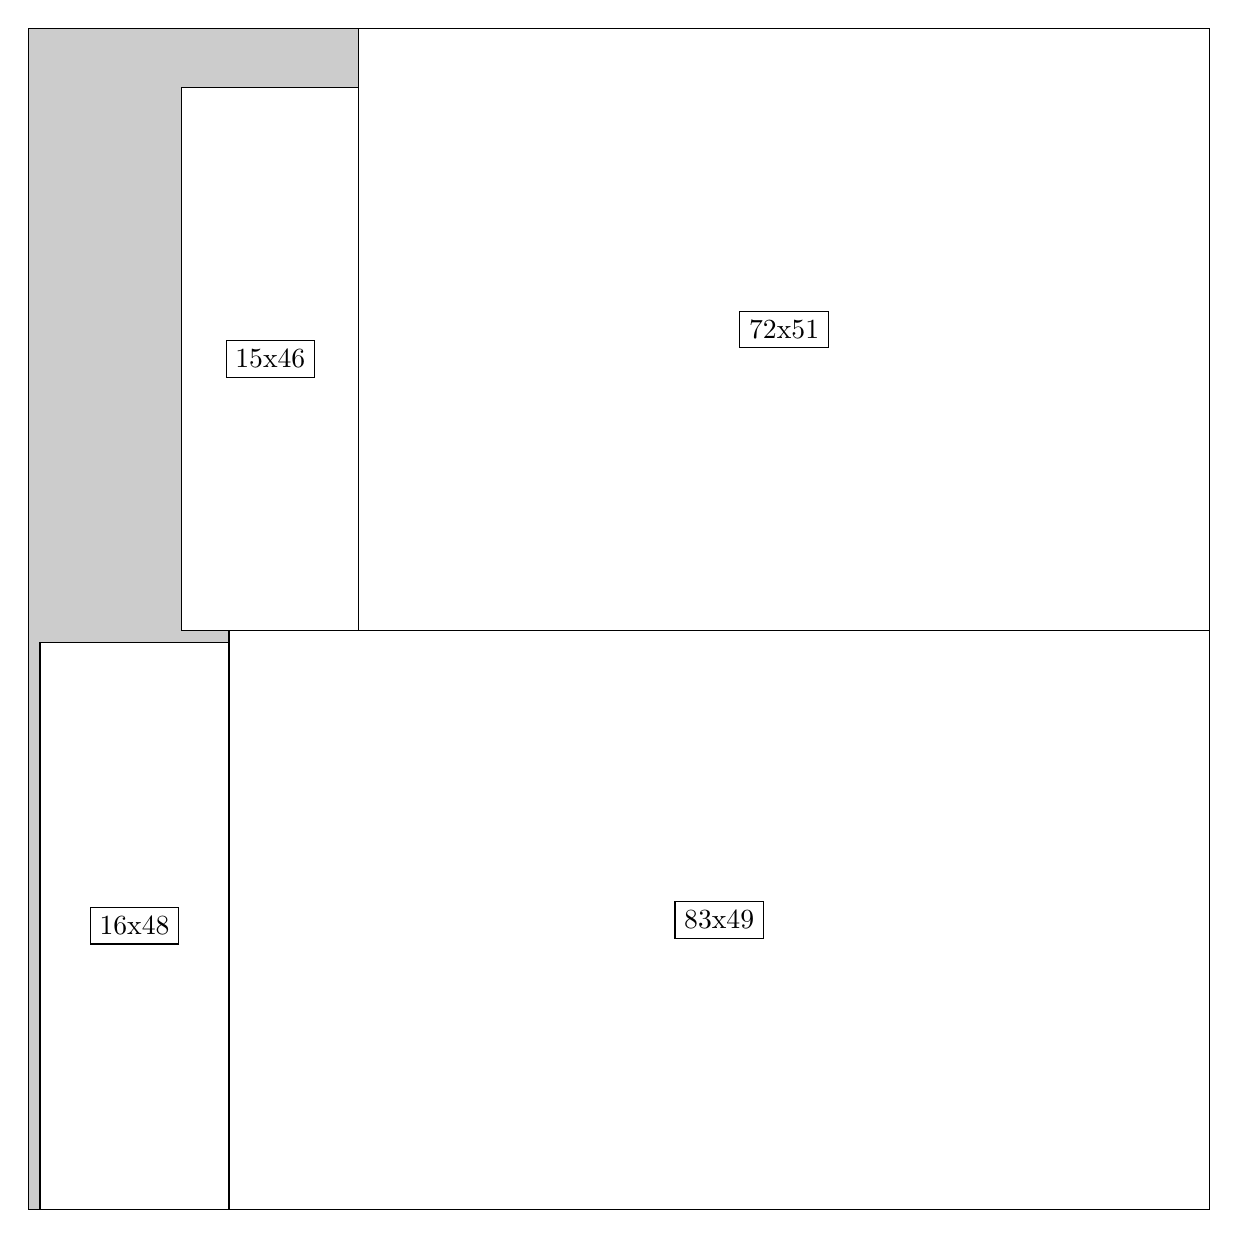
\begin{tikzpicture}[shorten >=1pt,scale=1.0,every node/.style={scale=1.0},->]
\tikzstyle{vertex}=[circle,fill=black!25,minimum size=14pt,inner sep=0pt]
\filldraw[fill=gray!40!white, draw=black] (0,0) rectangle (15.0,15.0);
\foreach \name/\x/\y/\w/\h in {83x49/2.55/0.0/12.45/7.35,16x48/0.15/0.0/2.4/7.199999999999999,72x51/4.2/7.35/10.799999999999999/7.6499999999999995,15x46/1.95/7.35/2.25/6.8999999999999995}
\filldraw[fill=white!40!white, draw=black] (\x,\y) rectangle node[draw] (\name) {\name} ++(\w,\h);
\end{tikzpicture}


w =83 , h =49 , x =17 , y =0 , v =4067
\par
w =16 , h =48 , x =1 , y =0 , v =768
\par
w =72 , h =51 , x =28 , y =49 , v =3672
\par
w =15 , h =46 , x =13 , y =49 , v =690
\par
\newpage


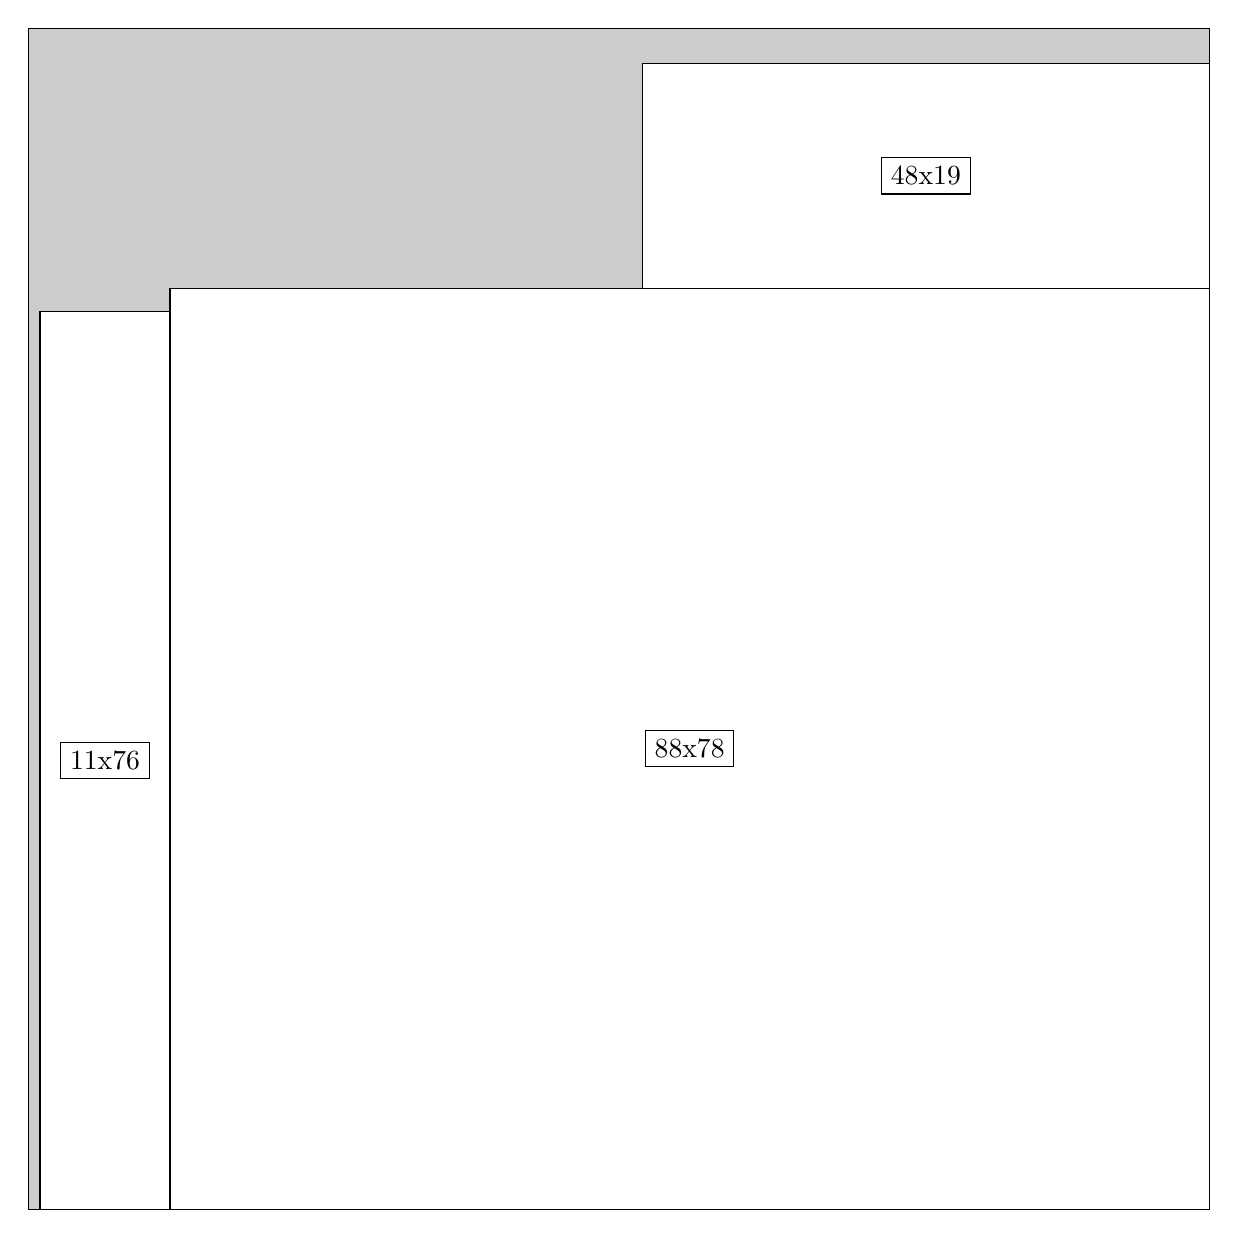
\begin{tikzpicture}[shorten >=1pt,scale=1.0,every node/.style={scale=1.0},->]
\tikzstyle{vertex}=[circle,fill=black!25,minimum size=14pt,inner sep=0pt]
\filldraw[fill=gray!40!white, draw=black] (0,0) rectangle (15.0,15.0);
\foreach \name/\x/\y/\w/\h in {88x78/1.7999999999999998/0.0/13.2/11.7,11x76/0.15/0.0/1.65/11.4,48x19/7.8/11.7/7.199999999999999/2.85}
\filldraw[fill=white!40!white, draw=black] (\x,\y) rectangle node[draw] (\name) {\name} ++(\w,\h);
\end{tikzpicture}


w =88 , h =78 , x =12 , y =0 , v =6864
\par
w =11 , h =76 , x =1 , y =0 , v =836
\par
w =48 , h =19 , x =52 , y =78 , v =912
\par
\newpage


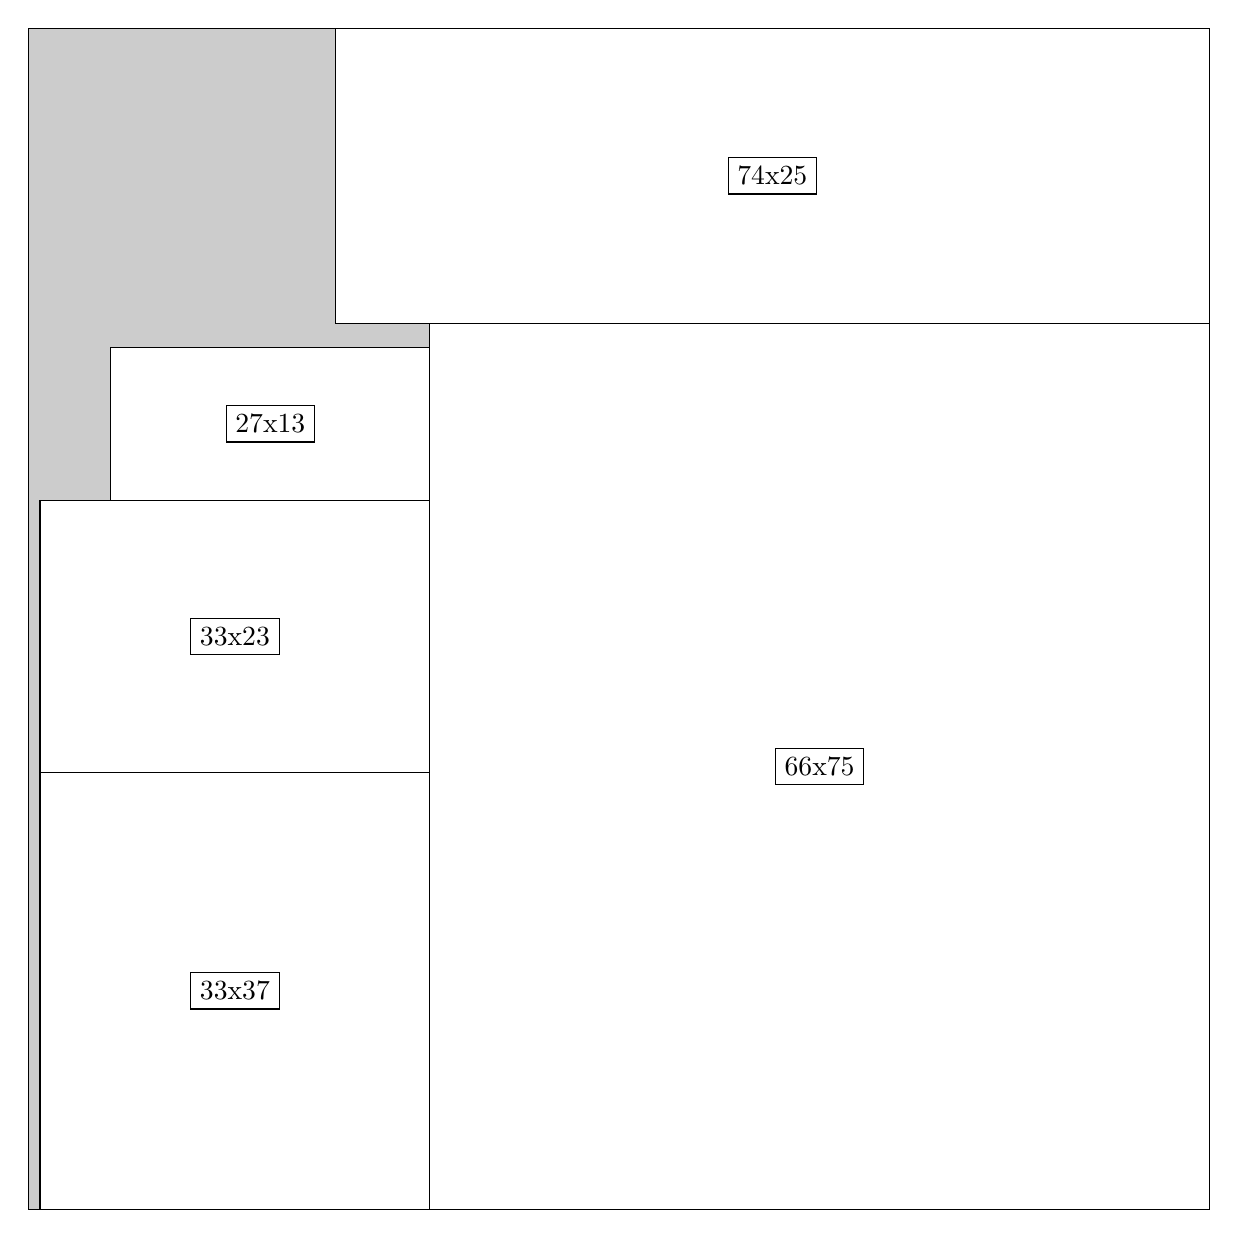
\begin{tikzpicture}[shorten >=1pt,scale=1.0,every node/.style={scale=1.0},->]
\tikzstyle{vertex}=[circle,fill=black!25,minimum size=14pt,inner sep=0pt]
\filldraw[fill=gray!40!white, draw=black] (0,0) rectangle (15.0,15.0);
\foreach \name/\x/\y/\w/\h in {66x75/5.1/0.0/9.9/11.25,33x37/0.15/0.0/4.95/5.55,33x23/0.15/5.55/4.95/3.4499999999999997,27x13/1.05/9.0/4.05/1.95,74x25/3.9/11.25/11.1/3.75}
\filldraw[fill=white!40!white, draw=black] (\x,\y) rectangle node[draw] (\name) {\name} ++(\w,\h);
\end{tikzpicture}


w =66 , h =75 , x =34 , y =0 , v =4950
\par
w =33 , h =37 , x =1 , y =0 , v =1221
\par
w =33 , h =23 , x =1 , y =37 , v =759
\par
w =27 , h =13 , x =7 , y =60 , v =351
\par
w =74 , h =25 , x =26 , y =75 , v =1850
\par
\newpage


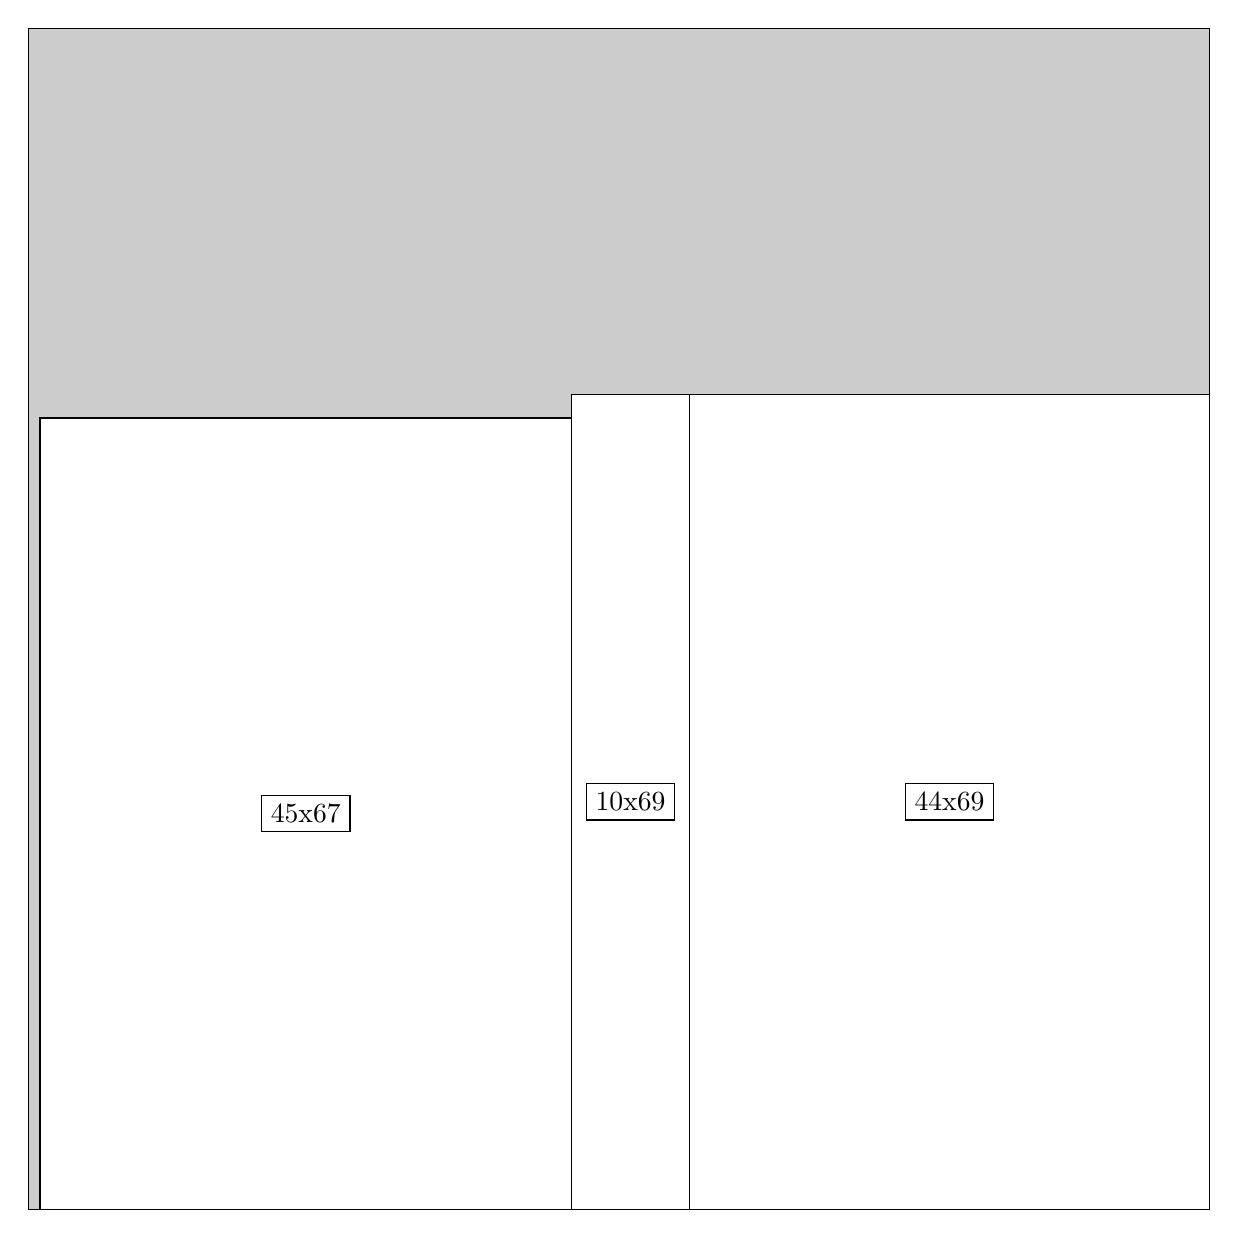
\begin{tikzpicture}[shorten >=1pt,scale=1.0,every node/.style={scale=1.0},->]
\tikzstyle{vertex}=[circle,fill=black!25,minimum size=14pt,inner sep=0pt]
\filldraw[fill=gray!40!white, draw=black] (0,0) rectangle (15.0,15.0);
\foreach \name/\x/\y/\w/\h in {44x69/8.4/0.0/6.6/10.35,10x69/6.8999999999999995/0.0/1.5/10.35,45x67/0.15/0.0/6.75/10.049999999999999}
\filldraw[fill=white!40!white, draw=black] (\x,\y) rectangle node[draw] (\name) {\name} ++(\w,\h);
\end{tikzpicture}


w =44 , h =69 , x =56 , y =0 , v =3036
\par
w =10 , h =69 , x =46 , y =0 , v =690
\par
w =45 , h =67 , x =1 , y =0 , v =3015
\par
\newpage


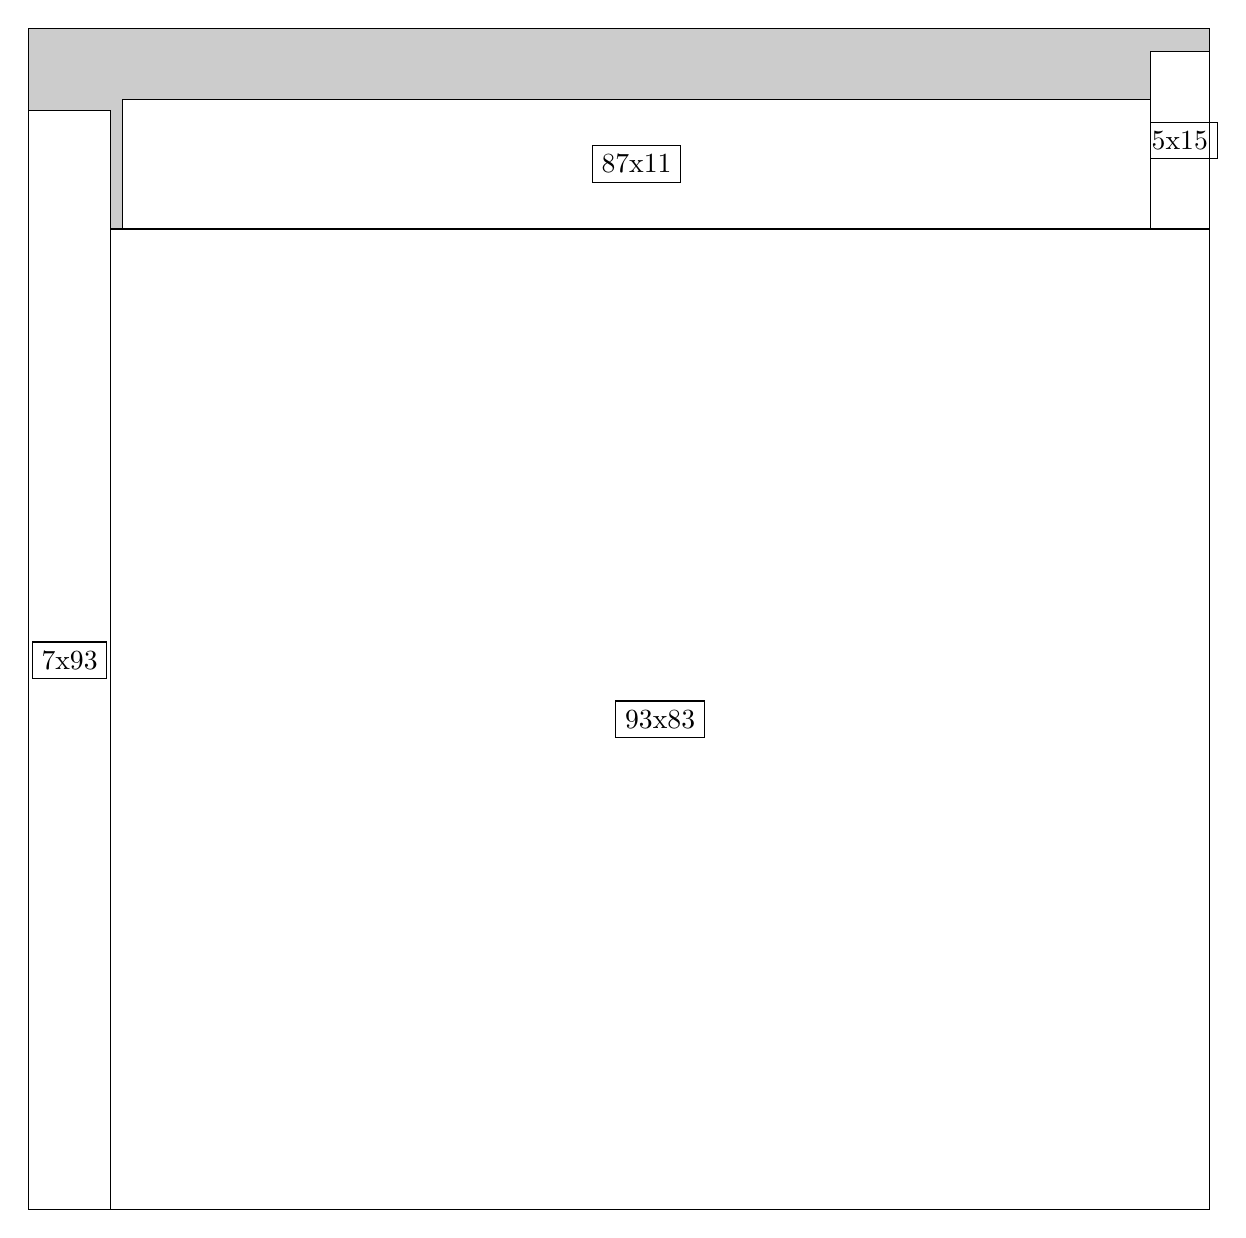
\begin{tikzpicture}[shorten >=1pt,scale=1.0,every node/.style={scale=1.0},->]
\tikzstyle{vertex}=[circle,fill=black!25,minimum size=14pt,inner sep=0pt]
\filldraw[fill=gray!40!white, draw=black] (0,0) rectangle (15.0,15.0);
\foreach \name/\x/\y/\w/\h in {93x83/1.05/0.0/13.95/12.45,5x15/14.25/12.45/0.75/2.25,87x11/1.2/12.45/13.049999999999999/1.65,7x93/0.0/0.0/1.05/13.95}
\filldraw[fill=white!40!white, draw=black] (\x,\y) rectangle node[draw] (\name) {\name} ++(\w,\h);
\end{tikzpicture}


w =93 , h =83 , x =7 , y =0 , v =7719
\par
w =5 , h =15 , x =95 , y =83 , v =75
\par
w =87 , h =11 , x =8 , y =83 , v =957
\par
w =7 , h =93 , x =0 , y =0 , v =651
\par
\newpage


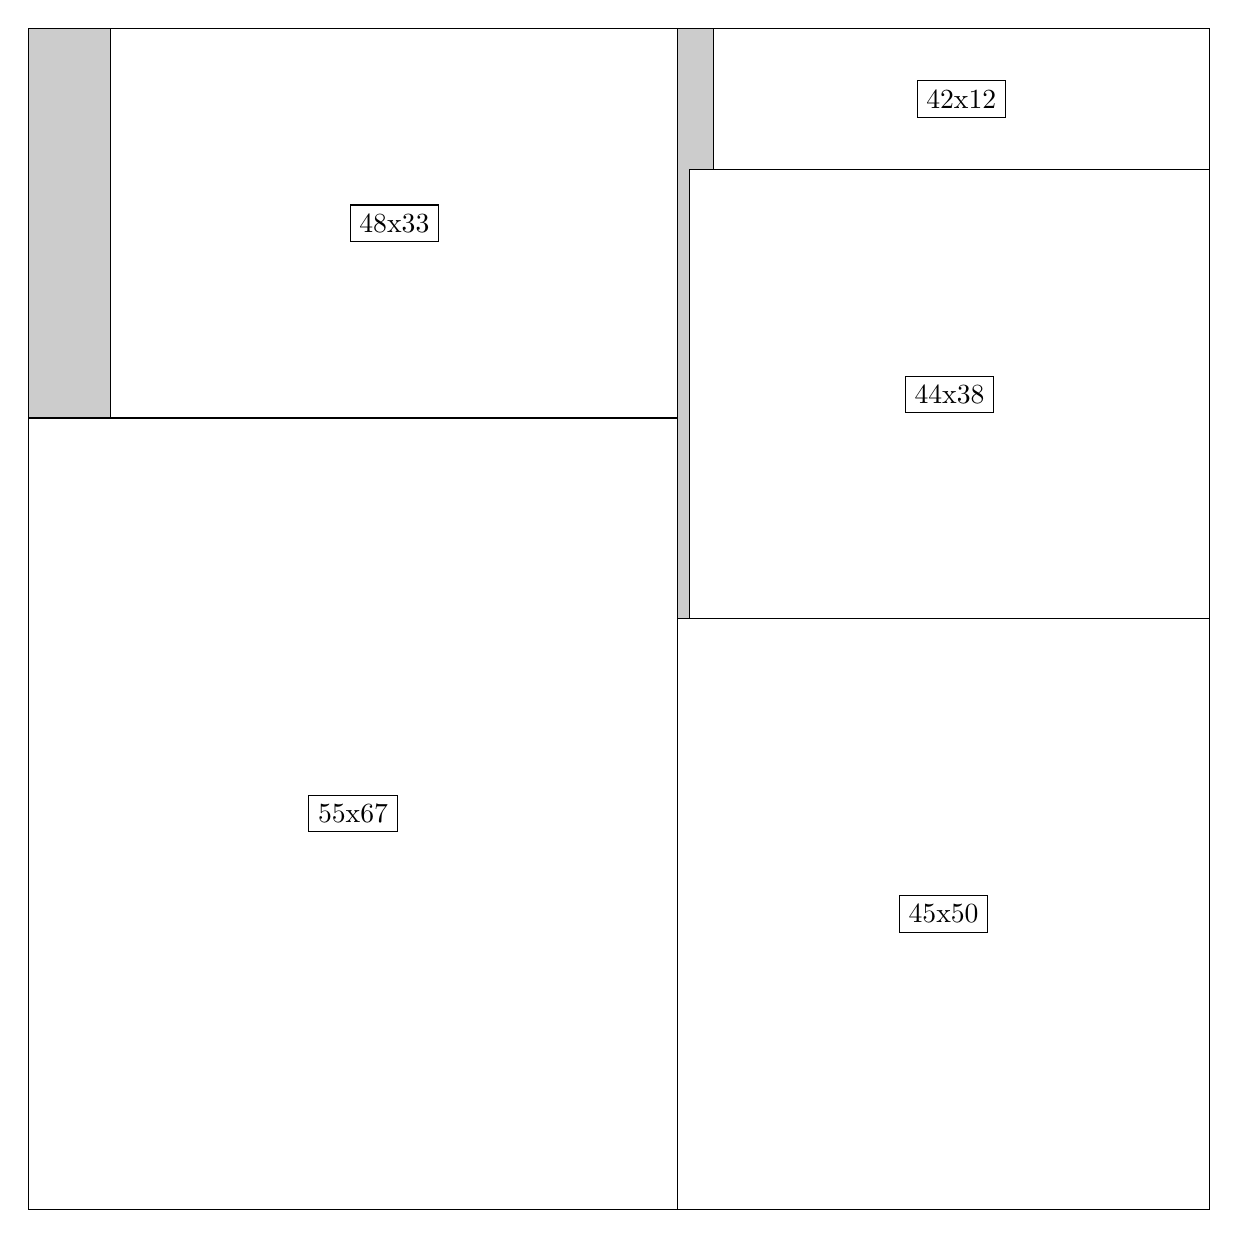
\begin{tikzpicture}[shorten >=1pt,scale=1.0,every node/.style={scale=1.0},->]
\tikzstyle{vertex}=[circle,fill=black!25,minimum size=14pt,inner sep=0pt]
\filldraw[fill=gray!40!white, draw=black] (0,0) rectangle (15.0,15.0);
\foreach \name/\x/\y/\w/\h in {45x50/8.25/0.0/6.75/7.5,44x38/8.4/7.5/6.6/5.7,42x12/8.7/13.2/6.3/1.7999999999999998,55x67/0.0/0.0/8.25/10.049999999999999,48x33/1.05/10.049999999999999/7.199999999999999/4.95}
\filldraw[fill=white!40!white, draw=black] (\x,\y) rectangle node[draw] (\name) {\name} ++(\w,\h);
\end{tikzpicture}


w =45 , h =50 , x =55 , y =0 , v =2250
\par
w =44 , h =38 , x =56 , y =50 , v =1672
\par
w =42 , h =12 , x =58 , y =88 , v =504
\par
w =55 , h =67 , x =0 , y =0 , v =3685
\par
w =48 , h =33 , x =7 , y =67 , v =1584
\par
\newpage


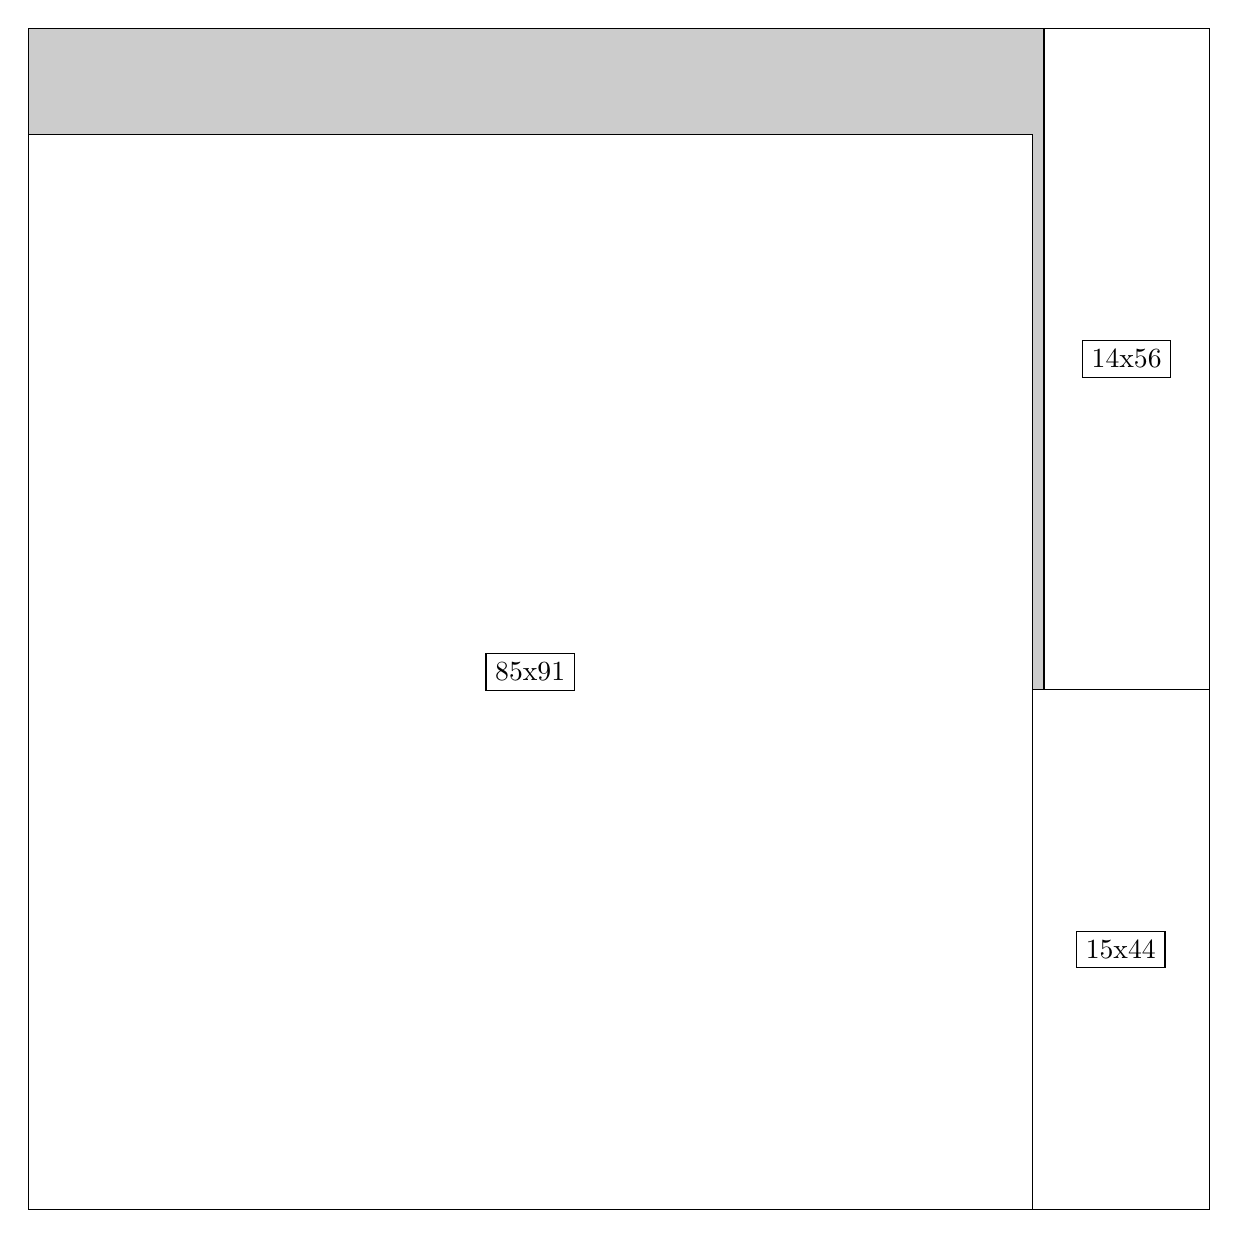
\begin{tikzpicture}[shorten >=1pt,scale=1.0,every node/.style={scale=1.0},->]
\tikzstyle{vertex}=[circle,fill=black!25,minimum size=14pt,inner sep=0pt]
\filldraw[fill=gray!40!white, draw=black] (0,0) rectangle (15.0,15.0);
\foreach \name/\x/\y/\w/\h in {15x44/12.75/0.0/2.25/6.6,14x56/12.9/6.6/2.1/8.4,85x91/0.0/0.0/12.75/13.65}
\filldraw[fill=white!40!white, draw=black] (\x,\y) rectangle node[draw] (\name) {\name} ++(\w,\h);
\end{tikzpicture}


w =15 , h =44 , x =85 , y =0 , v =660
\par
w =14 , h =56 , x =86 , y =44 , v =784
\par
w =85 , h =91 , x =0 , y =0 , v =7735
\par
\newpage


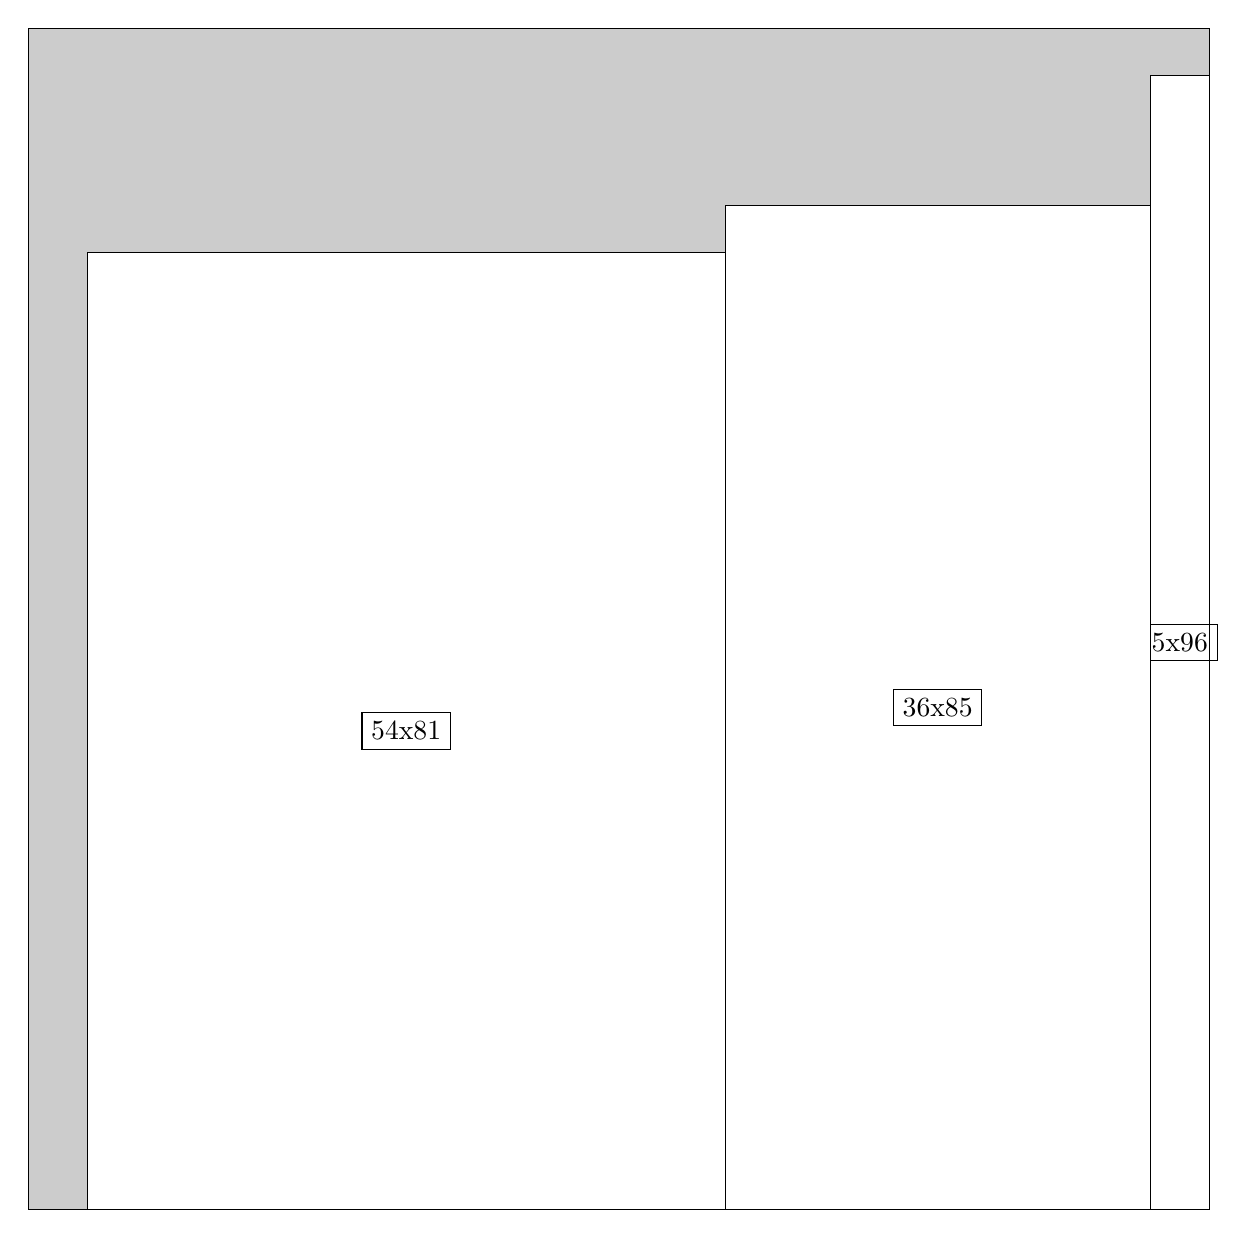
\begin{tikzpicture}[shorten >=1pt,scale=1.0,every node/.style={scale=1.0},->]
\tikzstyle{vertex}=[circle,fill=black!25,minimum size=14pt,inner sep=0pt]
\filldraw[fill=gray!40!white, draw=black] (0,0) rectangle (15.0,15.0);
\foreach \name/\x/\y/\w/\h in {5x96/14.25/0.0/0.75/14.399999999999999,36x85/8.85/0.0/5.3999999999999995/12.75,54x81/0.75/0.0/8.1/12.15}
\filldraw[fill=white!40!white, draw=black] (\x,\y) rectangle node[draw] (\name) {\name} ++(\w,\h);
\end{tikzpicture}


w =5 , h =96 , x =95 , y =0 , v =480
\par
w =36 , h =85 , x =59 , y =0 , v =3060
\par
w =54 , h =81 , x =5 , y =0 , v =4374
\par
\newpage


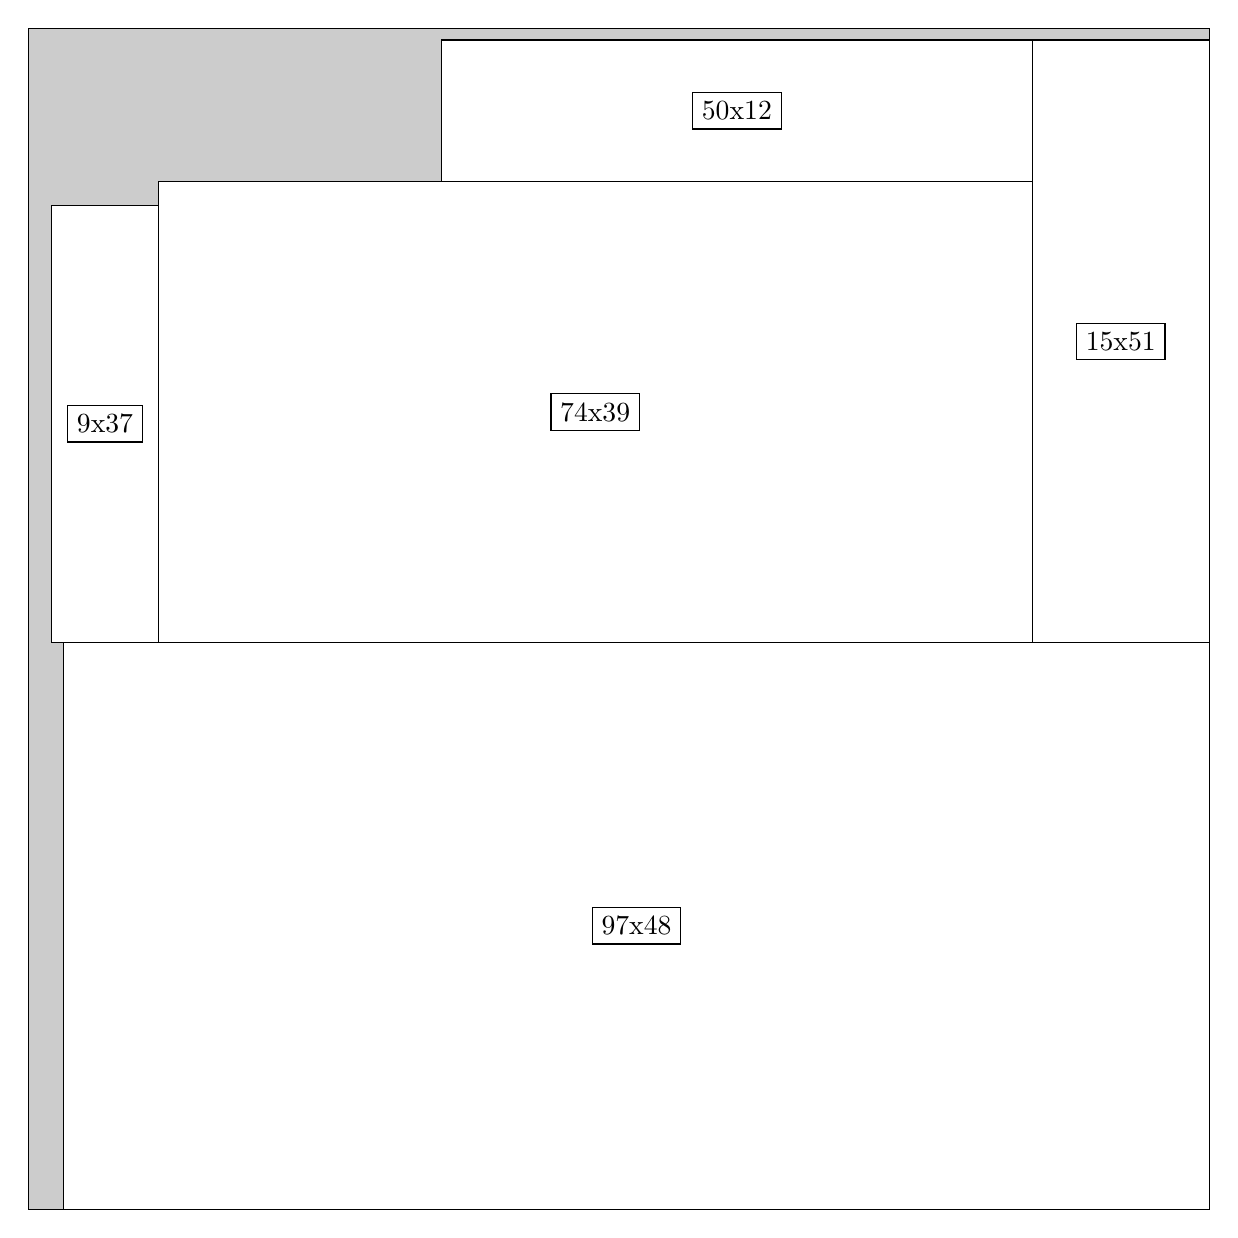
\begin{tikzpicture}[shorten >=1pt,scale=1.0,every node/.style={scale=1.0},->]
\tikzstyle{vertex}=[circle,fill=black!25,minimum size=14pt,inner sep=0pt]
\filldraw[fill=gray!40!white, draw=black] (0,0) rectangle (15.0,15.0);
\foreach \name/\x/\y/\w/\h in {97x48/0.44999999999999996/0.0/14.549999999999999/7.199999999999999,15x51/12.75/7.199999999999999/2.25/7.6499999999999995,74x39/1.65/7.199999999999999/11.1/5.85,50x12/5.25/13.049999999999999/7.5/1.7999999999999998,9x37/0.3/7.199999999999999/1.3499999999999999/5.55}
\filldraw[fill=white!40!white, draw=black] (\x,\y) rectangle node[draw] (\name) {\name} ++(\w,\h);
\end{tikzpicture}


w =97 , h =48 , x =3 , y =0 , v =4656
\par
w =15 , h =51 , x =85 , y =48 , v =765
\par
w =74 , h =39 , x =11 , y =48 , v =2886
\par
w =50 , h =12 , x =35 , y =87 , v =600
\par
w =9 , h =37 , x =2 , y =48 , v =333
\par
\newpage


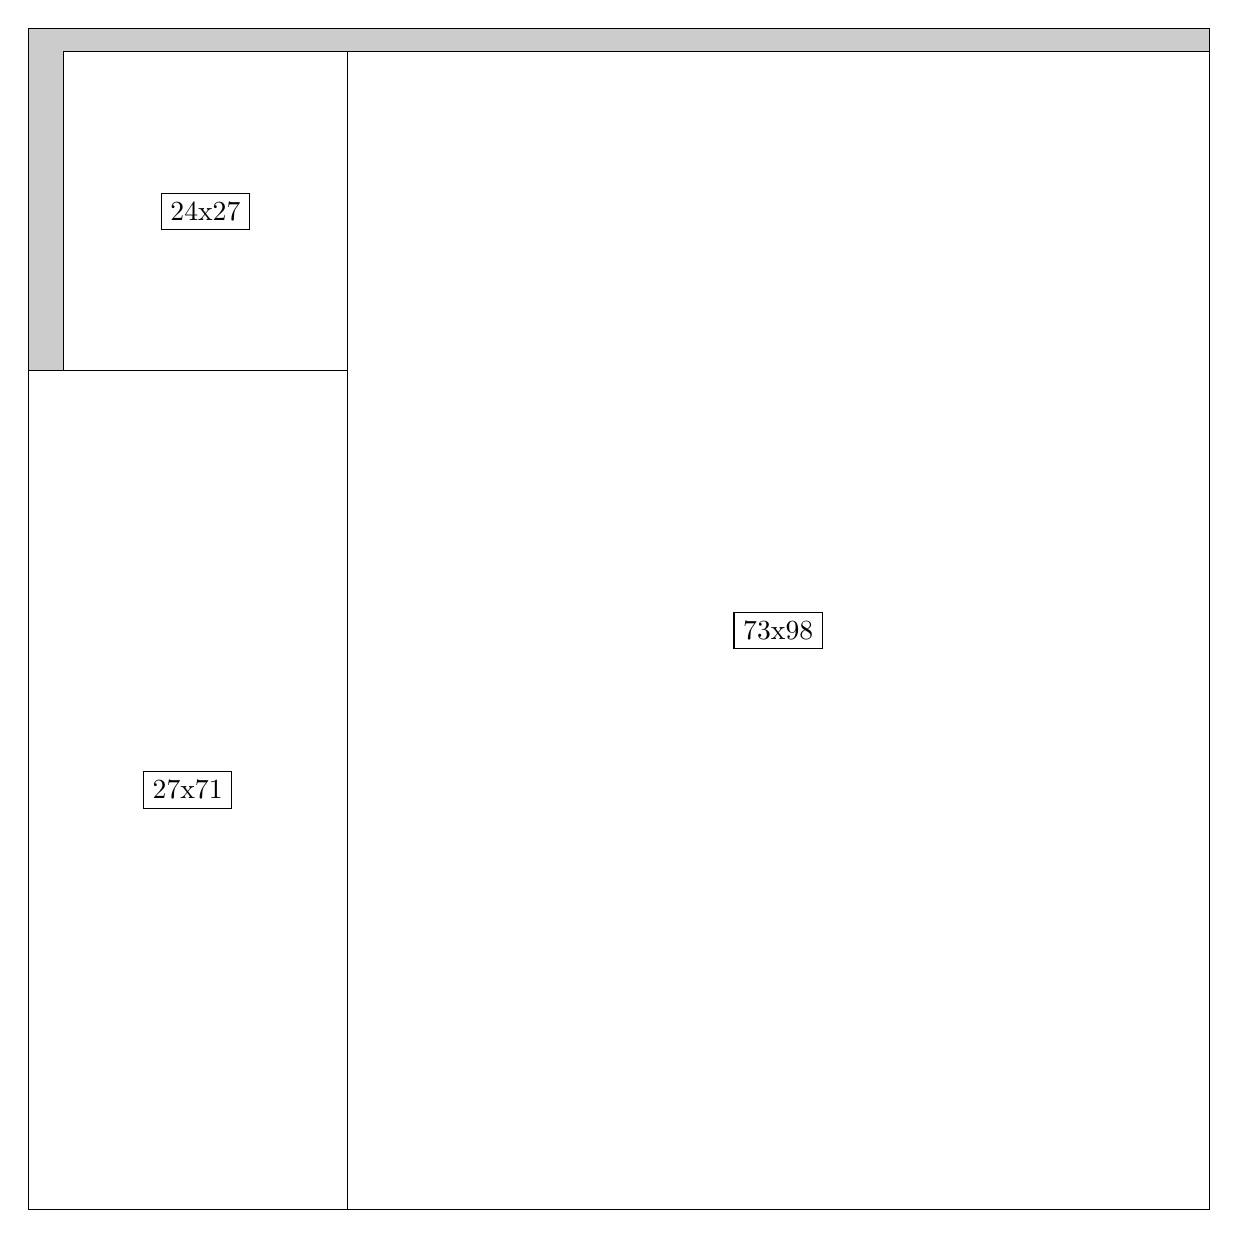
\begin{tikzpicture}[shorten >=1pt,scale=1.0,every node/.style={scale=1.0},->]
\tikzstyle{vertex}=[circle,fill=black!25,minimum size=14pt,inner sep=0pt]
\filldraw[fill=gray!40!white, draw=black] (0,0) rectangle (15.0,15.0);
\foreach \name/\x/\y/\w/\h in {73x98/4.05/0.0/10.95/14.7,27x71/0.0/0.0/4.05/10.65,24x27/0.44999999999999996/10.65/3.5999999999999996/4.05}
\filldraw[fill=white!40!white, draw=black] (\x,\y) rectangle node[draw] (\name) {\name} ++(\w,\h);
\end{tikzpicture}


w =73 , h =98 , x =27 , y =0 , v =7154
\par
w =27 , h =71 , x =0 , y =0 , v =1917
\par
w =24 , h =27 , x =3 , y =71 , v =648
\par
\newpage


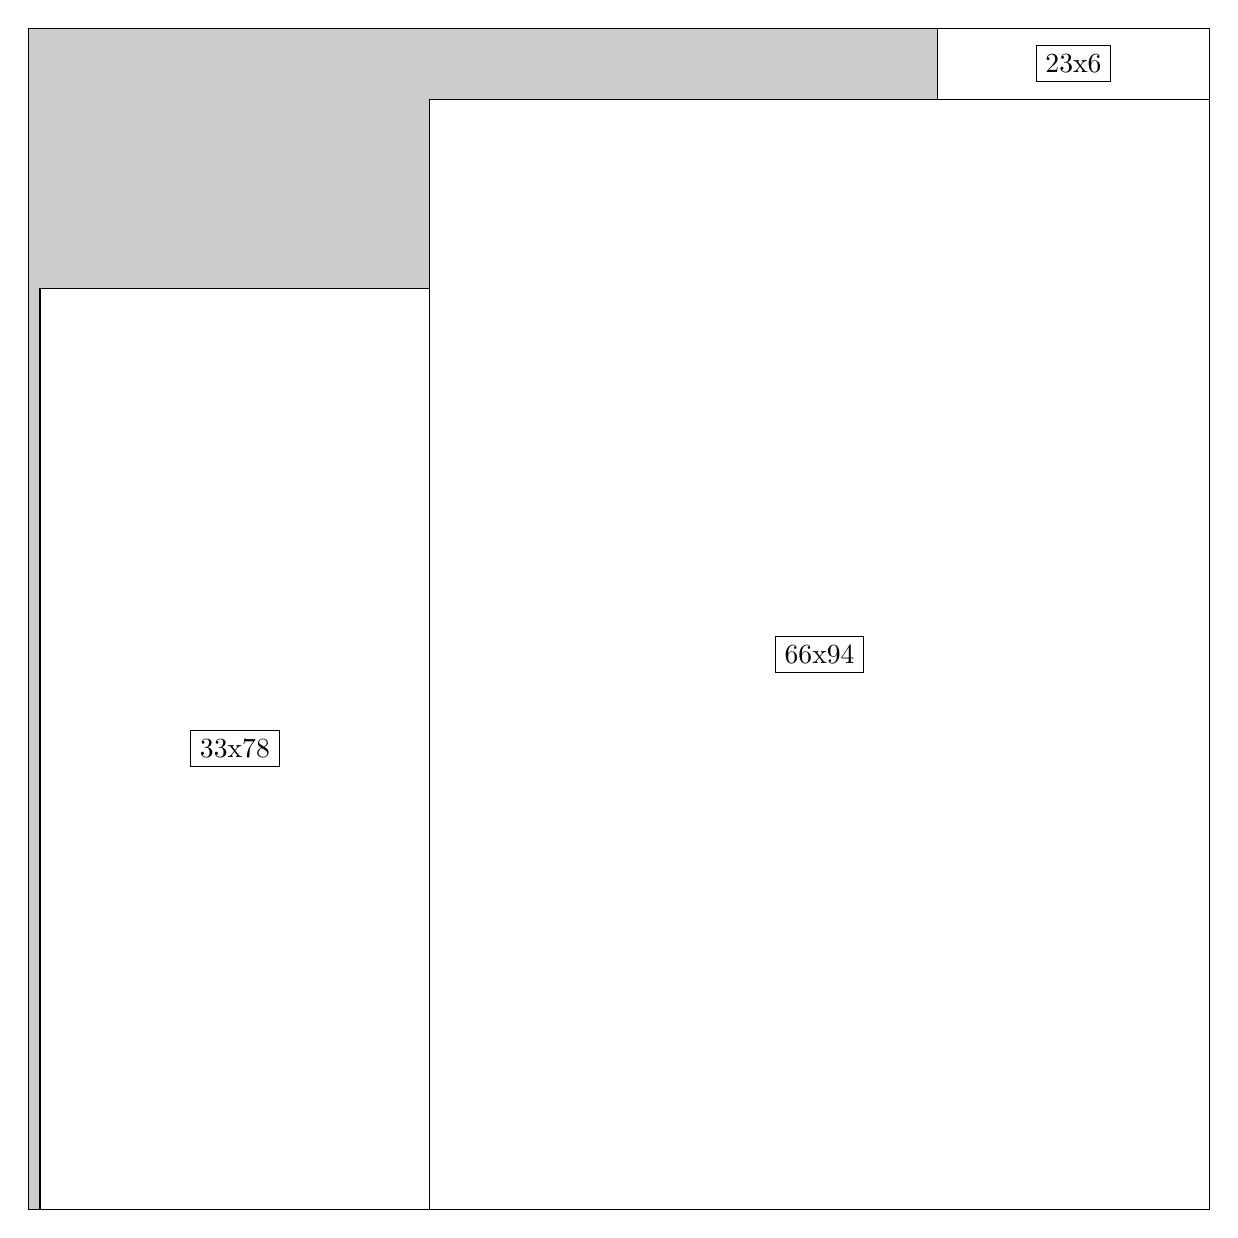
\begin{tikzpicture}[shorten >=1pt,scale=1.0,every node/.style={scale=1.0},->]
\tikzstyle{vertex}=[circle,fill=black!25,minimum size=14pt,inner sep=0pt]
\filldraw[fill=gray!40!white, draw=black] (0,0) rectangle (15.0,15.0);
\foreach \name/\x/\y/\w/\h in {66x94/5.1/0.0/9.9/14.1,23x6/11.549999999999999/14.1/3.4499999999999997/0.8999999999999999,33x78/0.15/0.0/4.95/11.7}
\filldraw[fill=white!40!white, draw=black] (\x,\y) rectangle node[draw] (\name) {\name} ++(\w,\h);
\end{tikzpicture}


w =66 , h =94 , x =34 , y =0 , v =6204
\par
w =23 , h =6 , x =77 , y =94 , v =138
\par
w =33 , h =78 , x =1 , y =0 , v =2574
\par
\newpage


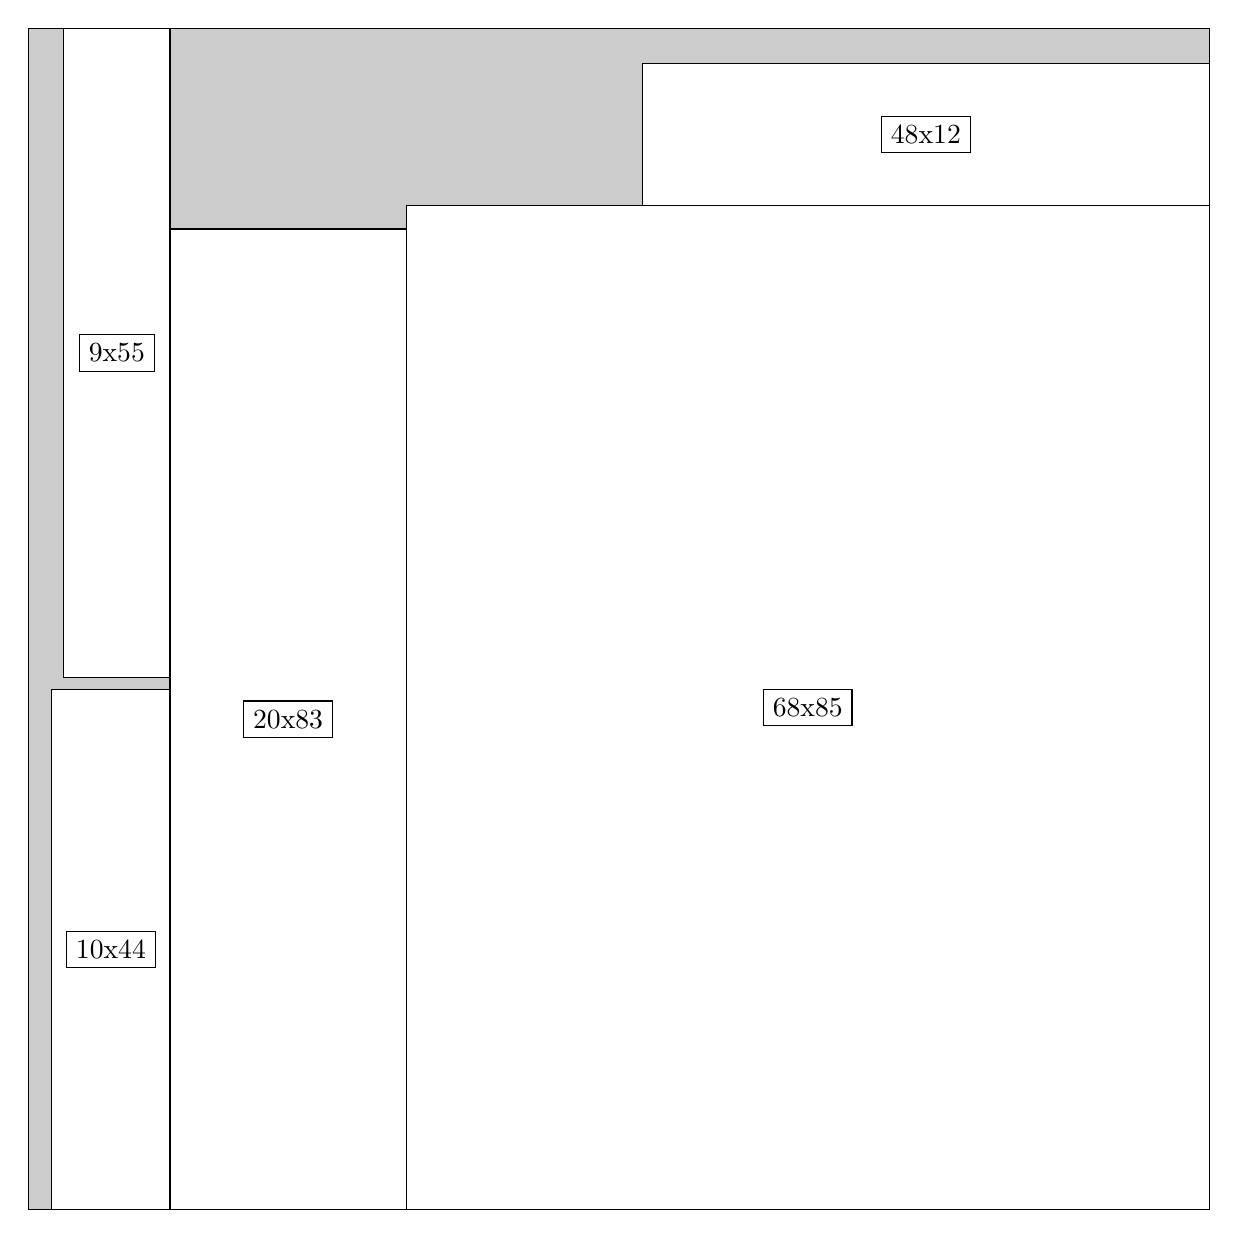
\begin{tikzpicture}[shorten >=1pt,scale=1.0,every node/.style={scale=1.0},->]
\tikzstyle{vertex}=[circle,fill=black!25,minimum size=14pt,inner sep=0pt]
\filldraw[fill=gray!40!white, draw=black] (0,0) rectangle (15.0,15.0);
\foreach \name/\x/\y/\w/\h in {68x85/4.8/0.0/10.2/12.75,48x12/7.8/12.75/7.199999999999999/1.7999999999999998,20x83/1.7999999999999998/0.0/3.0/12.45,10x44/0.3/0.0/1.5/6.6,9x55/0.44999999999999996/6.75/1.3499999999999999/8.25}
\filldraw[fill=white!40!white, draw=black] (\x,\y) rectangle node[draw] (\name) {\name} ++(\w,\h);
\end{tikzpicture}


w =68 , h =85 , x =32 , y =0 , v =5780
\par
w =48 , h =12 , x =52 , y =85 , v =576
\par
w =20 , h =83 , x =12 , y =0 , v =1660
\par
w =10 , h =44 , x =2 , y =0 , v =440
\par
w =9 , h =55 , x =3 , y =45 , v =495
\par
\newpage


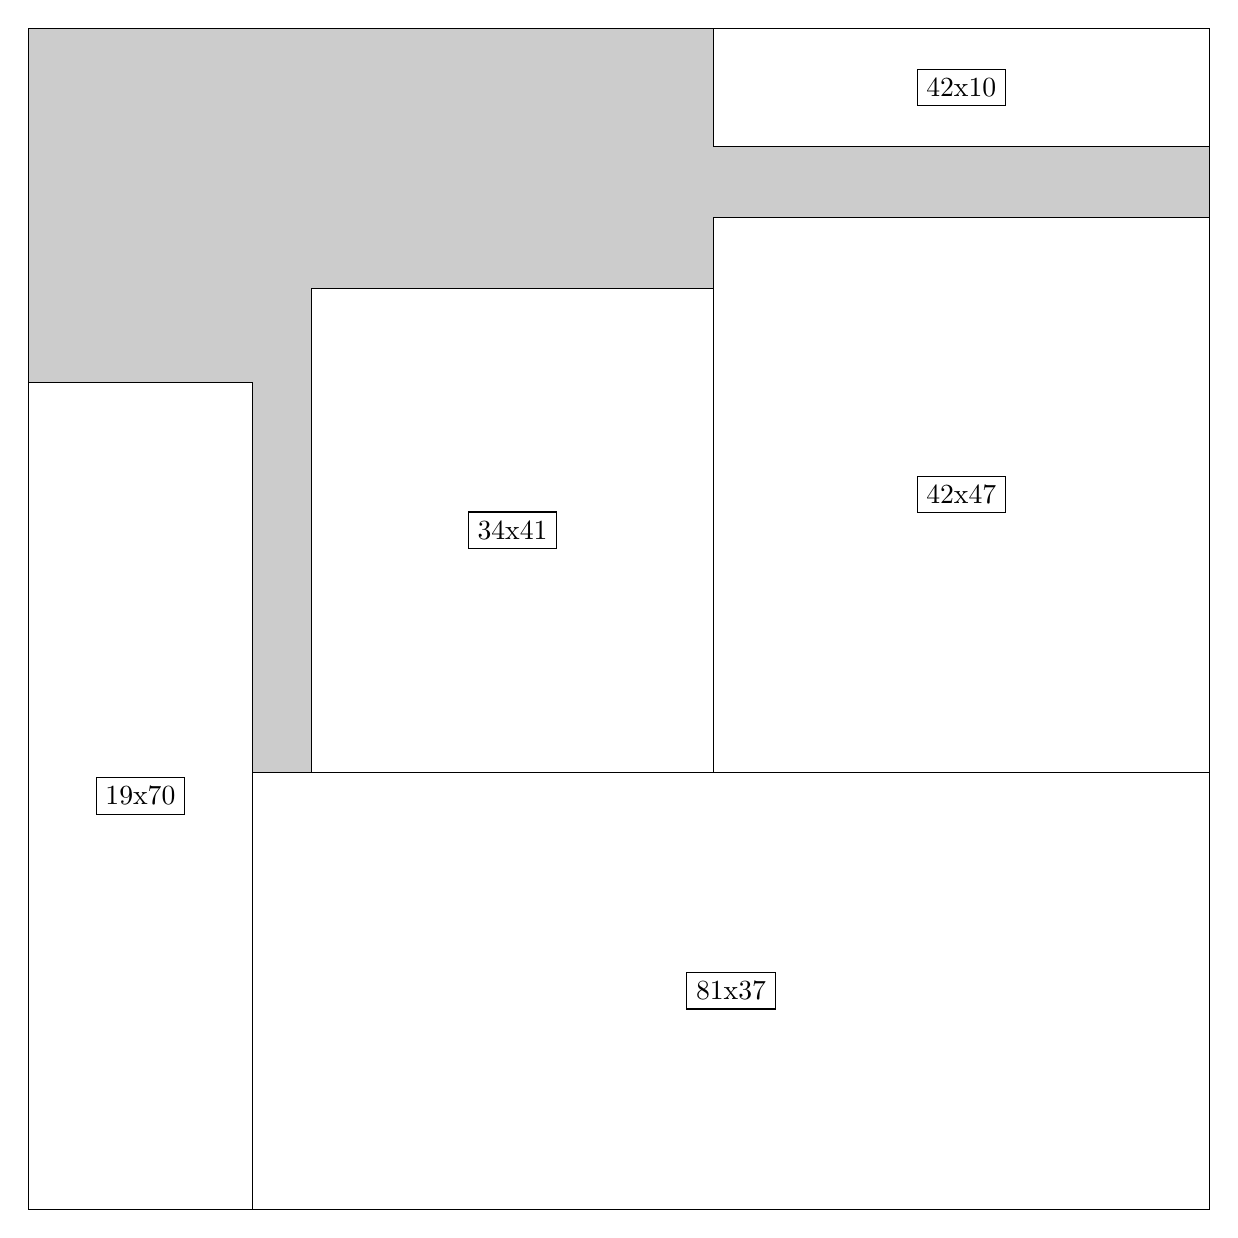
\begin{tikzpicture}[shorten >=1pt,scale=1.0,every node/.style={scale=1.0},->]
\tikzstyle{vertex}=[circle,fill=black!25,minimum size=14pt,inner sep=0pt]
\filldraw[fill=gray!40!white, draw=black] (0,0) rectangle (15.0,15.0);
\foreach \name/\x/\y/\w/\h in {81x37/2.85/0.0/12.15/5.55,42x47/8.7/5.55/6.3/7.05,34x41/3.5999999999999996/5.55/5.1/6.1499999999999995,42x10/8.7/13.5/6.3/1.5,19x70/0.0/0.0/2.85/10.5}
\filldraw[fill=white!40!white, draw=black] (\x,\y) rectangle node[draw] (\name) {\name} ++(\w,\h);
\end{tikzpicture}


w =81 , h =37 , x =19 , y =0 , v =2997
\par
w =42 , h =47 , x =58 , y =37 , v =1974
\par
w =34 , h =41 , x =24 , y =37 , v =1394
\par
w =42 , h =10 , x =58 , y =90 , v =420
\par
w =19 , h =70 , x =0 , y =0 , v =1330
\par
\newpage



\begin{tikzpicture}[shorten >=1pt,scale=1.0,every node/.style={scale=1.0},->]
\tikzstyle{vertex}=[circle,fill=black!25,minimum size=14pt,inner sep=0pt]
\filldraw[fill=gray!40!white, draw=black] (0,0) rectangle (15.0,15.0);
\foreach \name/\x/\y/\w/\h in {96x93/0.6/0.0/14.399999999999999/13.95}
\filldraw[fill=white!40!white, draw=black] (\x,\y) rectangle node[draw] (\name) {\name} ++(\w,\h);
\end{tikzpicture}


w =96 , h =93 , x =4 , y =0 , v =8928
\par
\newpage


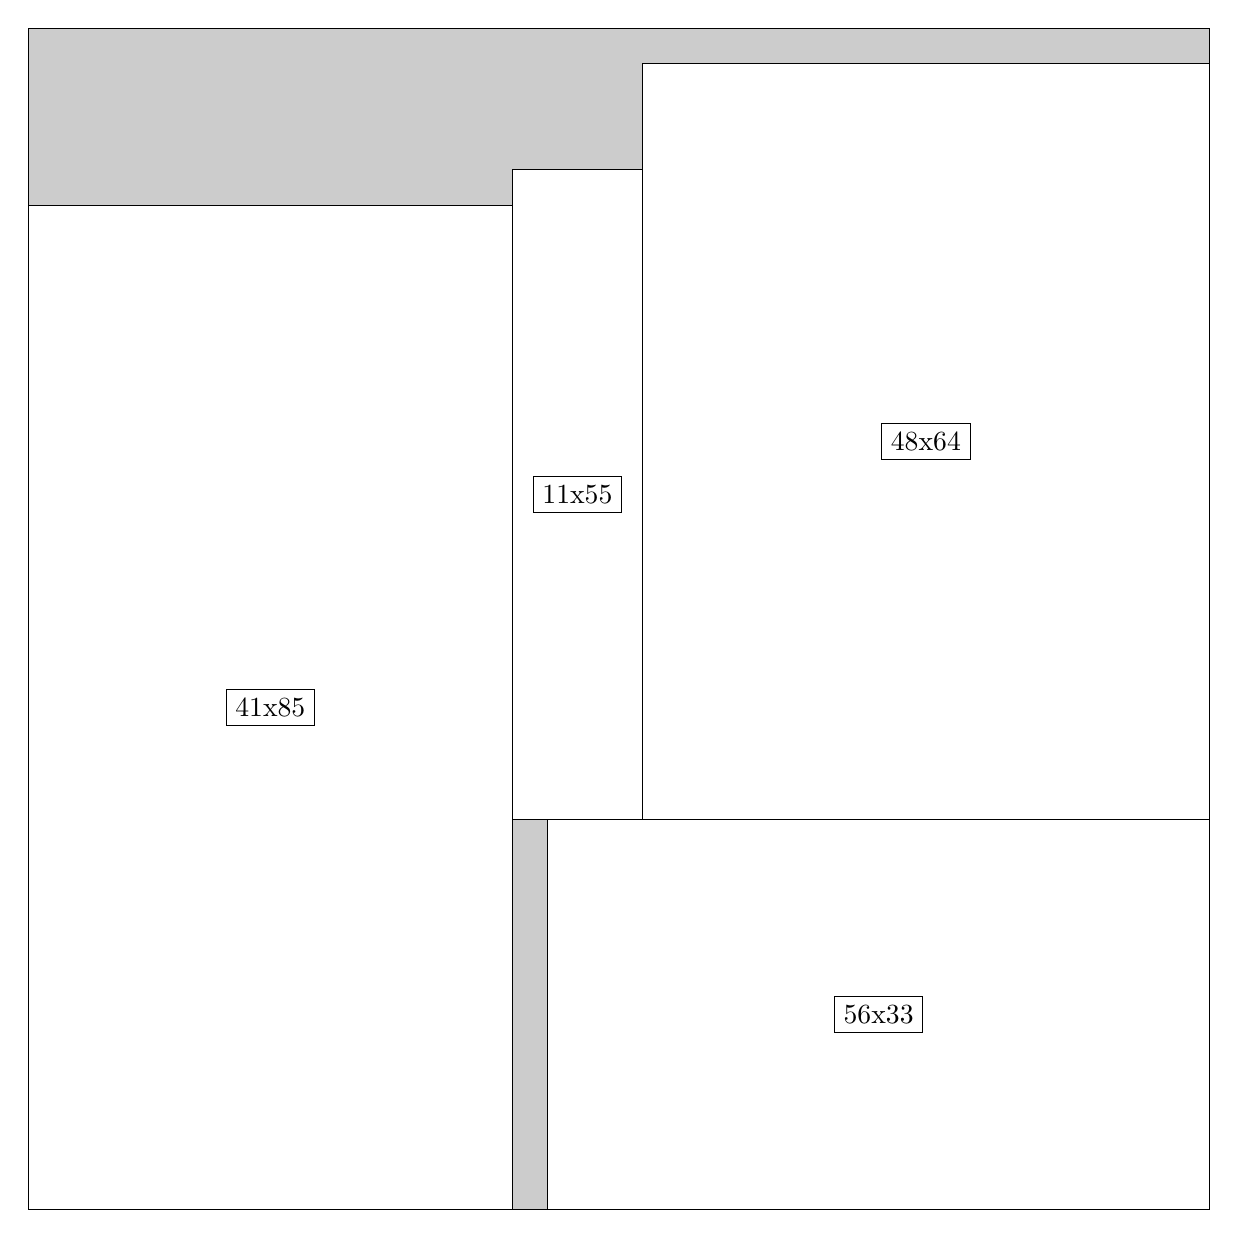
\begin{tikzpicture}[shorten >=1pt,scale=1.0,every node/.style={scale=1.0},->]
\tikzstyle{vertex}=[circle,fill=black!25,minimum size=14pt,inner sep=0pt]
\filldraw[fill=gray!40!white, draw=black] (0,0) rectangle (15.0,15.0);
\foreach \name/\x/\y/\w/\h in {56x33/6.6/0.0/8.4/4.95,48x64/7.8/4.95/7.199999999999999/9.6,11x55/6.1499999999999995/4.95/1.65/8.25,41x85/0.0/0.0/6.1499999999999995/12.75}
\filldraw[fill=white!40!white, draw=black] (\x,\y) rectangle node[draw] (\name) {\name} ++(\w,\h);
\end{tikzpicture}


w =56 , h =33 , x =44 , y =0 , v =1848
\par
w =48 , h =64 , x =52 , y =33 , v =3072
\par
w =11 , h =55 , x =41 , y =33 , v =605
\par
w =41 , h =85 , x =0 , y =0 , v =3485
\par
\newpage


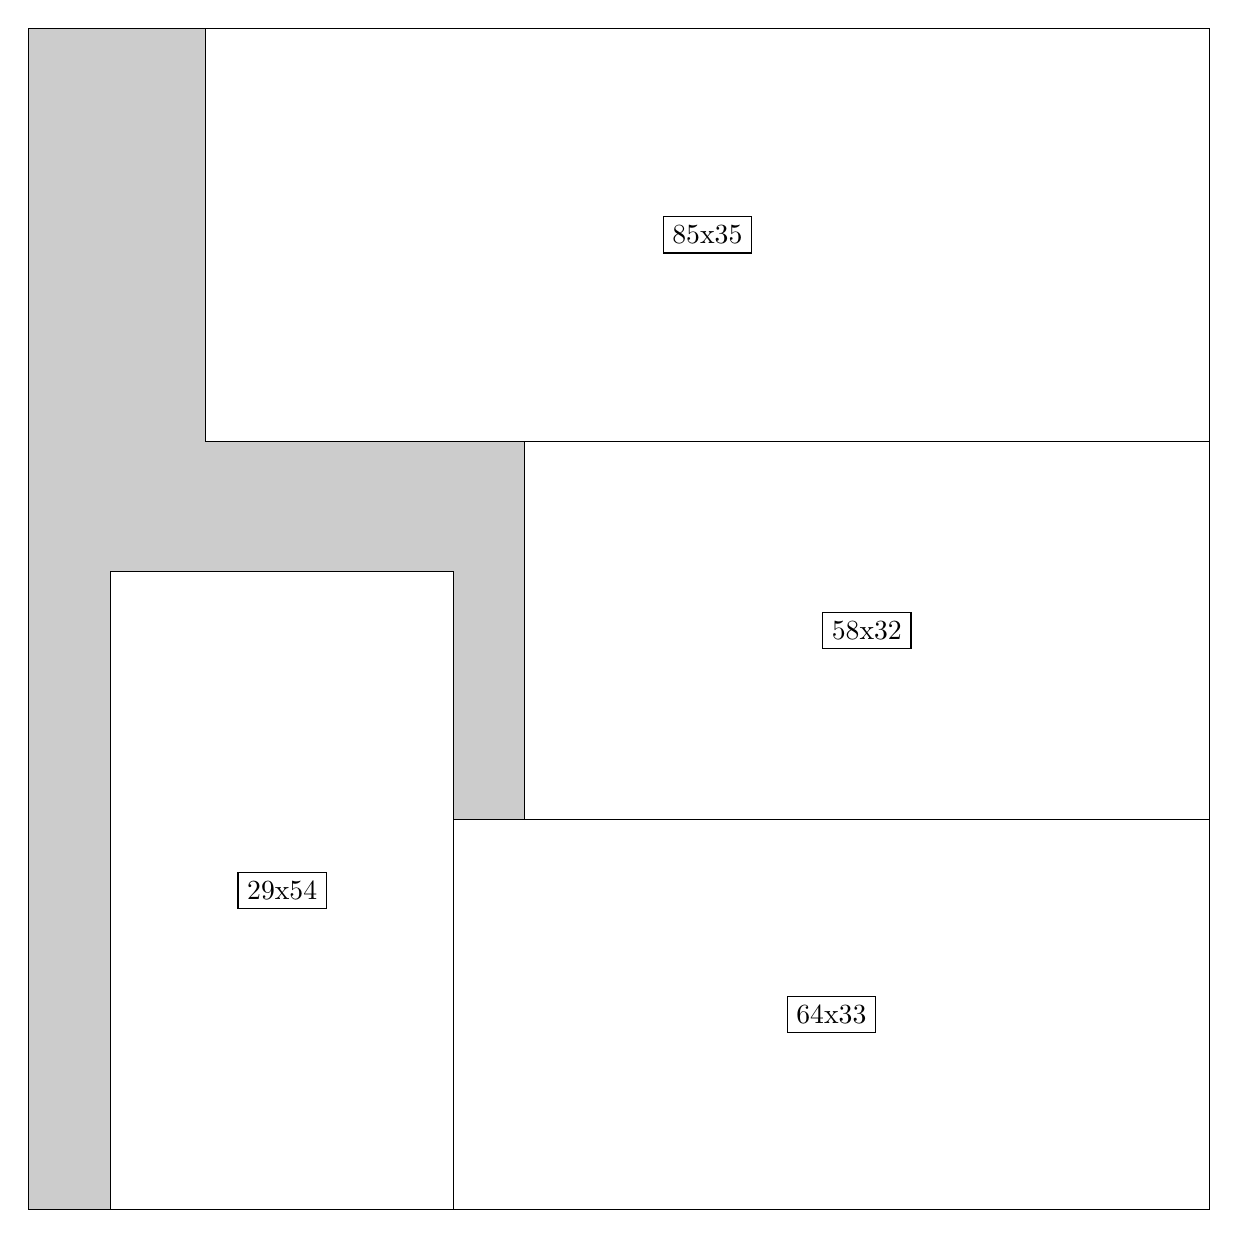
\begin{tikzpicture}[shorten >=1pt,scale=1.0,every node/.style={scale=1.0},->]
\tikzstyle{vertex}=[circle,fill=black!25,minimum size=14pt,inner sep=0pt]
\filldraw[fill=gray!40!white, draw=black] (0,0) rectangle (15.0,15.0);
\foreach \name/\x/\y/\w/\h in {64x33/5.3999999999999995/0.0/9.6/4.95,58x32/6.3/4.95/8.7/4.8,29x54/1.05/0.0/4.35/8.1,85x35/2.25/9.75/12.75/5.25}
\filldraw[fill=white!40!white, draw=black] (\x,\y) rectangle node[draw] (\name) {\name} ++(\w,\h);
\end{tikzpicture}


w =64 , h =33 , x =36 , y =0 , v =2112
\par
w =58 , h =32 , x =42 , y =33 , v =1856
\par
w =29 , h =54 , x =7 , y =0 , v =1566
\par
w =85 , h =35 , x =15 , y =65 , v =2975
\par
\newpage


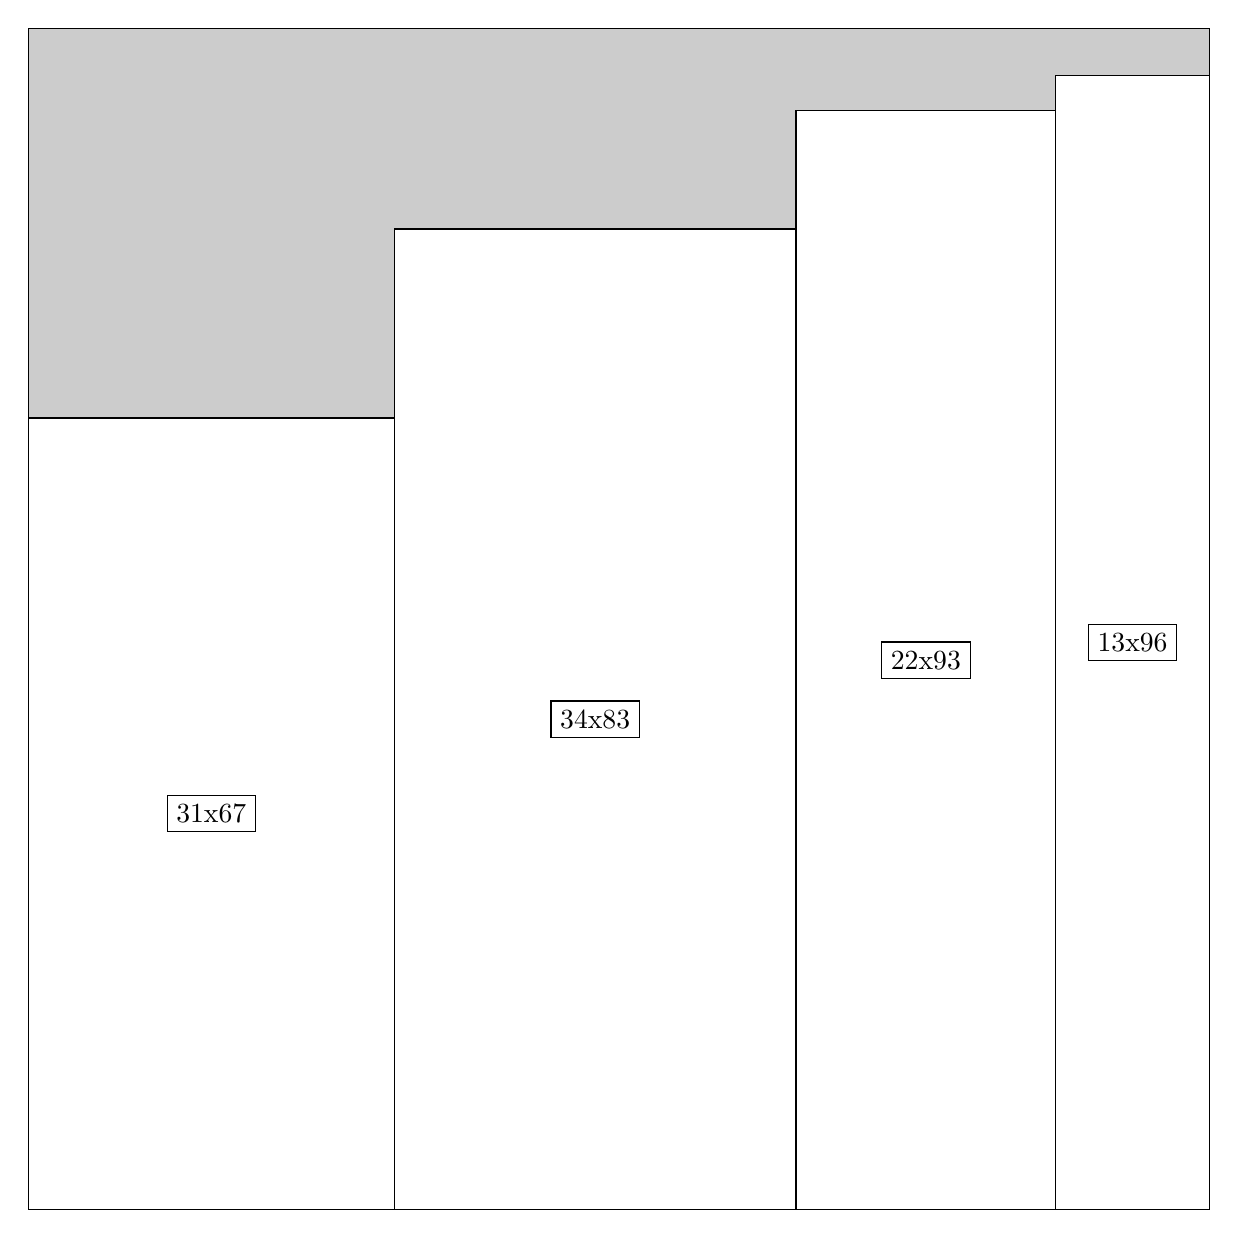
\begin{tikzpicture}[shorten >=1pt,scale=1.0,every node/.style={scale=1.0},->]
\tikzstyle{vertex}=[circle,fill=black!25,minimum size=14pt,inner sep=0pt]
\filldraw[fill=gray!40!white, draw=black] (0,0) rectangle (15.0,15.0);
\foreach \name/\x/\y/\w/\h in {13x96/13.049999999999999/0.0/1.95/14.399999999999999,22x93/9.75/0.0/3.3/13.95,34x83/4.6499999999999995/0.0/5.1/12.45,31x67/0.0/0.0/4.6499999999999995/10.049999999999999}
\filldraw[fill=white!40!white, draw=black] (\x,\y) rectangle node[draw] (\name) {\name} ++(\w,\h);
\end{tikzpicture}


w =13 , h =96 , x =87 , y =0 , v =1248
\par
w =22 , h =93 , x =65 , y =0 , v =2046
\par
w =34 , h =83 , x =31 , y =0 , v =2822
\par
w =31 , h =67 , x =0 , y =0 , v =2077
\par
\newpage


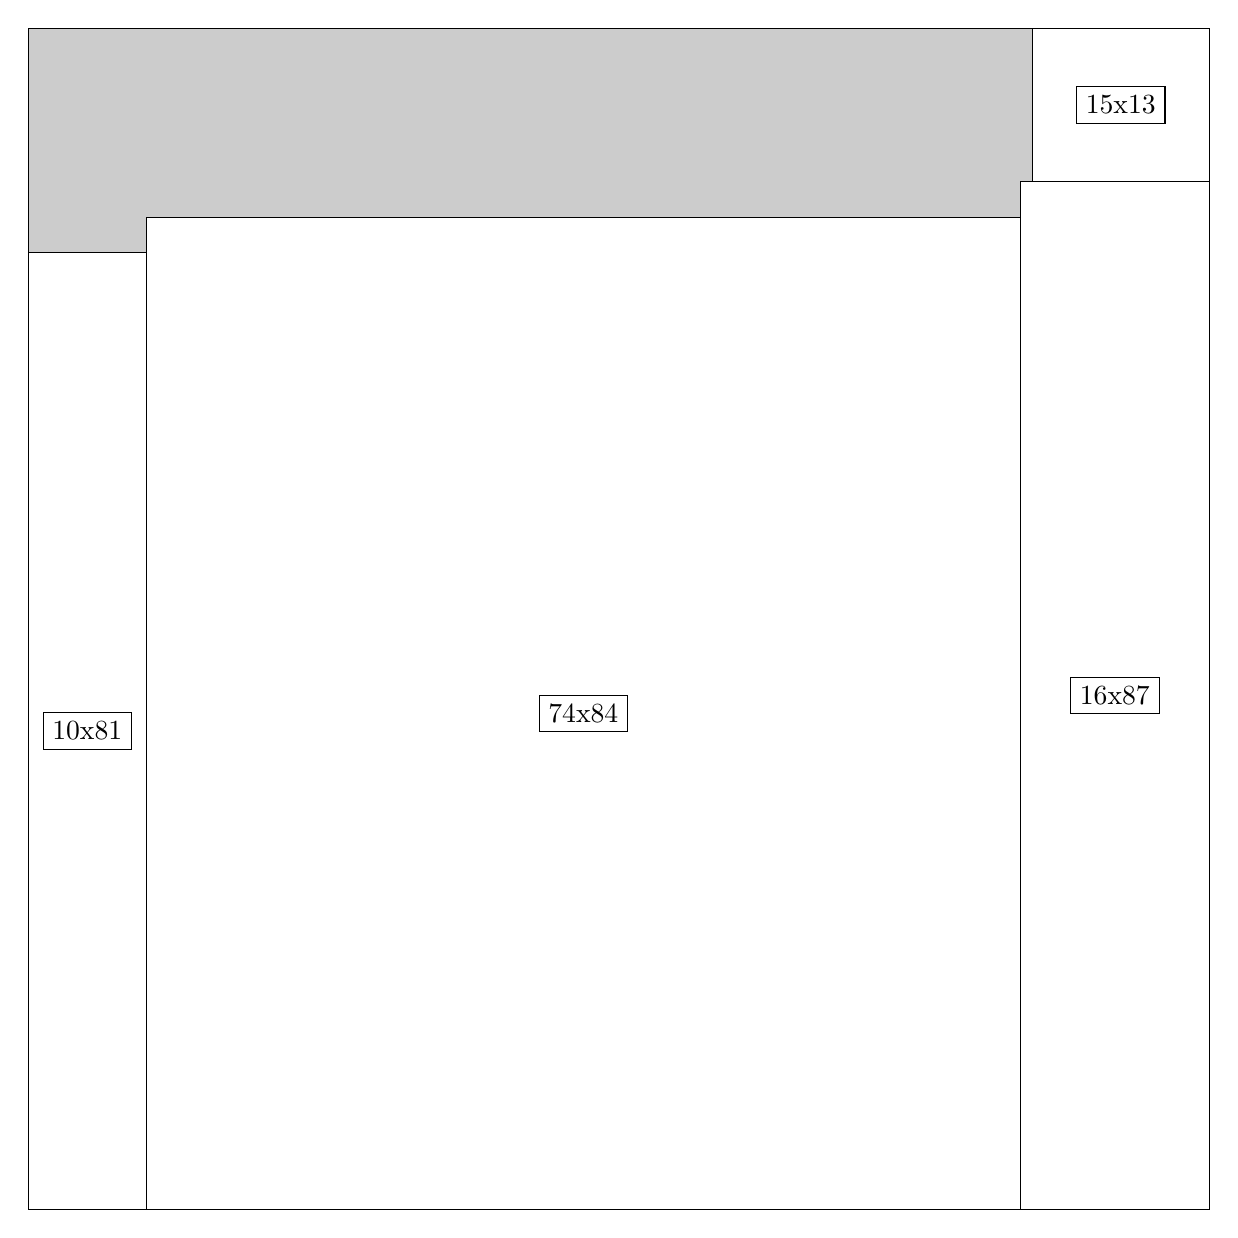
\begin{tikzpicture}[shorten >=1pt,scale=1.0,every node/.style={scale=1.0},->]
\tikzstyle{vertex}=[circle,fill=black!25,minimum size=14pt,inner sep=0pt]
\filldraw[fill=gray!40!white, draw=black] (0,0) rectangle (15.0,15.0);
\foreach \name/\x/\y/\w/\h in {16x87/12.6/0.0/2.4/13.049999999999999,15x13/12.75/13.049999999999999/2.25/1.95,74x84/1.5/0.0/11.1/12.6,10x81/0.0/0.0/1.5/12.15}
\filldraw[fill=white!40!white, draw=black] (\x,\y) rectangle node[draw] (\name) {\name} ++(\w,\h);
\end{tikzpicture}


w =16 , h =87 , x =84 , y =0 , v =1392
\par
w =15 , h =13 , x =85 , y =87 , v =195
\par
w =74 , h =84 , x =10 , y =0 , v =6216
\par
w =10 , h =81 , x =0 , y =0 , v =810
\par
\newpage


\end{document}